\label{chapter2}
A literature review is completed to gain a deeper understanding of the specified topic, provide insights on work previously done and identify key factors that need to be addressed. The contribution of this dissertation is given as the addition of an additional cost allocation method into a simulation tool as well as a further investigation into the practical implementation of collaborations to identify the limitations that hinder the incorporation of the model in real-life scenarios. Therefore, the literature review will focus on the research concerning the modelling of urban freight transportation as well as that of collaborations and the available infrastructure for developing these models.

\section{Defining Urban Freight Transportation}
Urban freight transportation is defined as the activities involved in providing citizens in urban areas with access to consumables and goods, at a specific location and time where it is required \citep{sonke2008the}. This traditional urban freight transportation definition and objective differs from that of sustainable urban freight transport. Sustainable urban freight transportation is defined as a system that contributes to the growth of the economy and social equity, while also focusing on the impact on the environment. Urban freight transport is a critical component in developing economic growth \citep{lindholm2012challenges}, as it contributes a significant proportion of the Gross Domestic Product (\acrshort{gdp}) \citep{makamo2015road}. However, little attention has been focused on enhancing the research on urban freight practices to convert the focus from the traditional objective, of only managing the movement of goods, towards a sustainable urban freight transport objective \citep{sonke2008the}. The continuous negative trend of implementing sustainable urban freight transportation is mainly due to the lack of prioritising the projects combined with the lack of awareness and knowledge in handling the problems \citep{behrends2008impact}.
%ADD RESEARCH ARTICLES THAT HAVE ADDRESSED THE INCLUSION OF SUSTAINABLE URBAN FREIGHT PRACTICES
The realisation of this focus shift has been gaining momentum in mega-cities around the world that are adapting and improving the culture for urban mobility \citep{lindholm2012challenges}.\par

The importance of this shift towards an improved and sustainable future in urban freight transport is considered as a necessary step \citep{savelsbergh201650th,macharis2014stakeholder,lindholm2012challenges} as external factors further increase the strain placed on urban freight transportation. A growing competitiveness in the market, have increased logistics costs as competitors attempt to gain market by introducing higher customer service levels \citep{lozano2013cooperative}. In turn, the direct-to-customer deliveries have increased drastically and although this compliments the unique needs of the customer, it increases the required number of freight movements \citep{savelsbergh201650th}. 

The demand for freight movement is generated by the actors in the supply chain. Various agents can participate in a given supply chain. The agents participating in the urban freight transportation sector are referred to as \textit{freight} agents. A widely known categorization class the different freight agents as the \textit{shipper} agent, the \textit{carrier} agent, the \textit{receiver} agent and the \textit{administrator} agent. The latter forms part of the public sector, whereas the shipper, carrier and receiver agents form part of the private sector. The freight agent categorisation used in this dissertation is shown in figure \ref{agent_interact}.

\begin{figure}[ht]
    \centering
    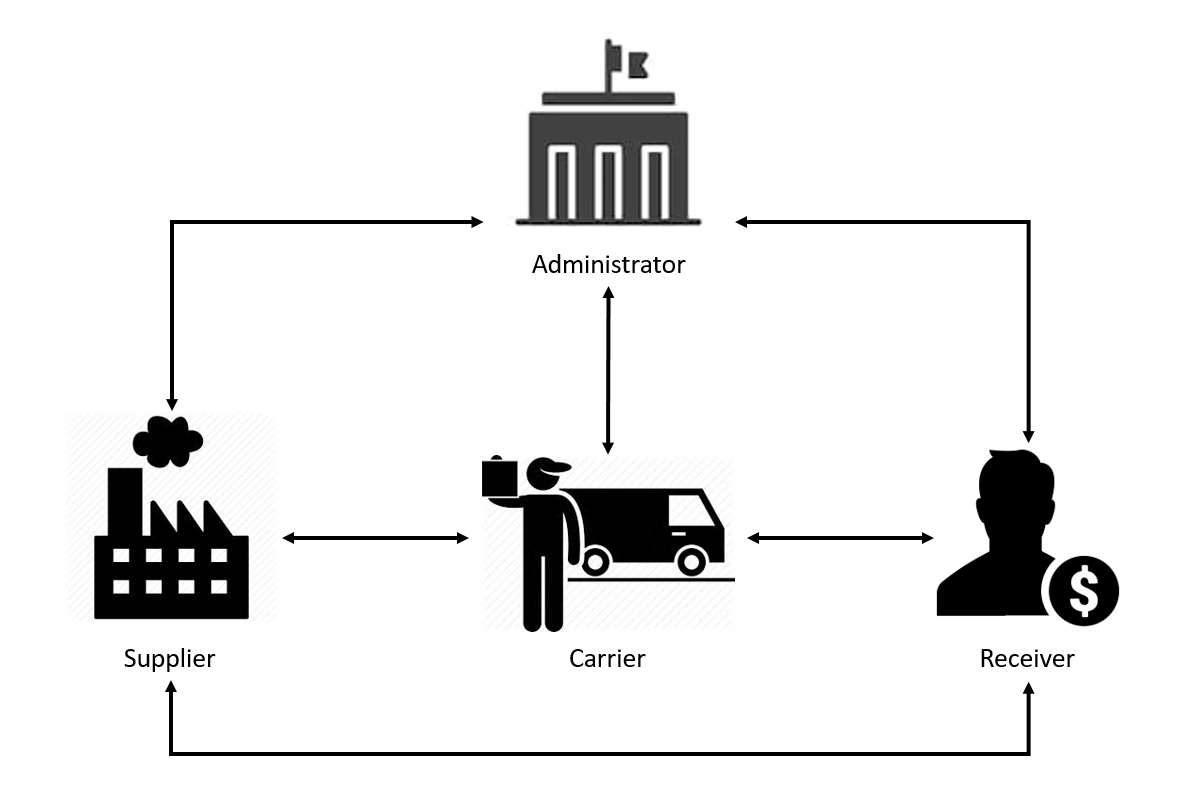
\includegraphics{images/agent_interact.PNG}
    \caption{Agent categorisation and interaction links}
    \label{agent_interact}
\end{figure}

\begin{enumerate}
    \item The \textit{shipper} agent is the owner of the product. This agent is responsible for supplying the product into the supply chain. The shipper agent has three interactions. The interactions with other agent types influence the decisions made by the shipper agent. Infrastructure available and policies such as product regulations or safety regulations introduced by the administrator agent has an impact on the decisions made by the shipper agent. This describes the administrator-shipper interaction. Vehicle type and availability of vehicles available to execute deliveries for the specific shipper agent are examples of the shipper-carrier interaction. The last interaction, known as the shipper-receiver interaction, determines the product and delivery requirements. The product specifications and required due date (or delivery date) are specified by the receiver agent.
    
    \item The \textit{carrier} agent is seen as the agent that transports the goods to the end customer. The responsibilities of the carrier can be executed in two manners. The shipper can act as the carrier, in this scenario the warehouse or factory uses private vehicles to distribute their goods and the carrier agent forms part of the supplier agent. On the other hand, the carrier agent can form part of an external third-party logistics provider. In this example, the warehouse or factory does not own a private fleet and has to make use of companies to distribute goods. Therefore, the carrier agent has three potential interactions. The first interaction is the administrator-carrier interaction. Available road infrastructure and the coupled condition of the available infrastructure affects the decisions made by the carrier. Another example of this interaction is the vehicle load regulations that affect the packing of the freight vehicle and the maximum load allowed per vehicle type. The shipper-carrier interaction provides the pick-up locations of goods and the number of goods to be delivered. The final interaction is the carrier-receiver interaction. This interaction affects the delivery schedule used by the carrier agent. Receiver locations and delivery specifications are specified by the receiver agent.
    
    \item The \textit{receiver} agent acts as the end-user of the goods. This can either be a retail store or consumer. The receiver agent has three potential interactions. Similar to the shipper and carrier agents, the receiver agent interacts with the administrator agent as regulations and policies are introduced by the administrator agent. The receiver communicates the product requirements, preferred delivery due date and delivery specifications to the shipper agent. The carrier-receiver interaction describes the physical delivery of goods at the specified receiver location.
    
    \item The \textit{administrator} agent provides the infrastructure on which the other freight agents execute their daily activities. The main responsibility of these agents is to uphold an economical and environmentally friendly city environment by implementing certain measures and policies. An example of an administrator agent is the municipality \citep{anand2014ontology}. The administrator interacts with all three of the private sector agents. Factors such as toll gate rates, road maintenance, vehicle loading regulations and product regulations are examples of decisions made by this agent that affect the other agents in that area.
\end{enumerate}


An increase in logistic activities in urban areas has a direct negative impact on congestion, infrastructure deterioration, safety and environmental impacts such as emissions and other pollution forms \citep{lindawati2014collaboration,savelsbergh201650th, bean2018, gonzalez2012defining,savelsbergh201650th}.  To fully understand the factors that have led to this predicament, the negative impacts of increased urban freight movements are investigated. \par

From the perspective of the different agents involved, the negative impacts result in additional delivery costs incurred. The costs associated with completing a delivery includes a fixed cost component (given as R/day) and a variable cost component (given as R/km) \citep{bean2018}. These cost components depend on the vehicle type selected for the delivery route. Each vehicle type has different cost components. Heavy vehicle types tend to have higher cost components as it provides more capacity, allowing the transportation of more goods in a single delivery trip. The main congestion bottleneck is located in urban areas where the freight vehicles have to compete with other freight vehicles and private vehicles. External factors may result in additional costs being accumulated. Time plays an important role in the planning of urban freight vehicles and calculating the estimated delivery cost. The optimal planning of urban freight vehicles are obscured by the presence of other vehicles on the road that result in congestion and influence the planned time for a delivery. In order to obtain a realistic estimation of the total delivery cost incurred, the discussed variables should be included into the delivery cost calculation. \par
%INCLUDE AN ARTICLE THAT REALISED THE IMPORTANCE OF INCLUDING THE TIME FACTOR

Congestion, delays and deteriorated infrastructure are examples of additional costs being passed on to the shipper and carrier agents which further increases the total supply chain cost.  \citep{giuliano2013synthesis}. A delay in freight vehicles, result in a delay cost accumulated by the carrier and shipper agents \citep{giuliano2013synthesis} as the delivery is not completed in the specified time frame. These delivery time frames, specified by the receiver agent, set the period in which a receiver is willing to accept delivery. This period is referred to as the delivery time window. Furthermore, the cost of freight transport has increased in recent years due to the state of the road infrastructure. This results in increased maintenance and repair costs as well as the cost of lost goods due to accidents of freight vehicles \citep{havenga2011case}. Incorporating these external factors into the decision making process has encouraged the use of modelling techniques to assist in planning urban freight transport. \par

%Incorporating these external factors into the cost calculation has been known as being complex as the different variables are a function of time and is therefore difficult to estimate. From here research turned towards modelling these urban freight vehicles in order to accurately capture these estimates.

%PROVIDE RESEARCH ON MODELS THAT CALCULATED THE DELIVERY COST THROUGH ALGORITHMS< NORMAL CALCS?


\section{Modelling Urban Freight Transportation}

%\citet{joubert2010large} presents an article that focuses on modelling agent-based freight transportation scenarios in the Gauteng, South Africa area. 
The complexity of the supply chain, the large variety of products involved and the reliability of the data used, serves as reasons for the delayed development of freight transportation models found in the literature \citep{joubert2010large}. When referring to the modeling of urban freight transportation specifically, trip-based and activity-based models describe the two groups of modeling approaches. Each of these model types' origin and progress through the years are reviewed in the next section.

%This article presented the activity chains extracted from this raw data and would be the first integration of private car and freight agents found in literature \citep{horni2016multi}.


%The data used for the \textit{freight agent} plans, were derived from GPS records and included over 30 000 commercial vehicles. This represented an estimated 35\% of the total Gauteng commercial traffic.  

%Simulation describes a set of rules that describe how a certain system will change in the future, when given its present state \citep{borshchev2004system}.



%-------------------------------------------------------------------------------------------------------------

\subsection{Trip-based models}

The need for a travel and demand planning model has been recognized from as early as the mid-twentieth century. During this period of the 1950's a sequential modelling approach that could estimate the travel demand was introduced. This model was known as the four-stage model, as shown in figure \ref{fig:four_steps}, and it was originally used to model passenger flows \citep{sivakumar2007modelling}, but could also be applied to urban freight transportation scenarios \citep{deJong2014new}. 

\begin{figure}[h]
    \centering
    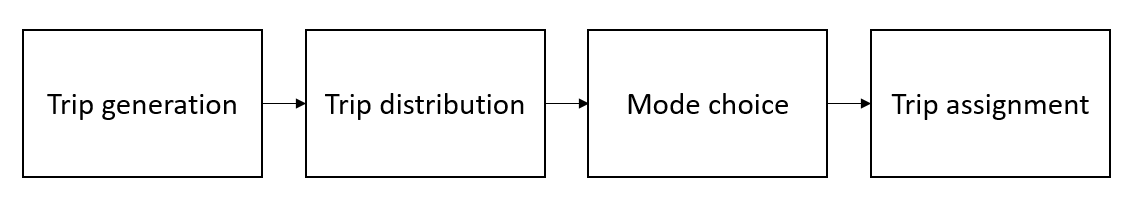
\includegraphics{images/four_step_model.PNG}
    \caption{The classical four-step modeling approach}
    \label{fig:four_steps}
\end{figure}

The discussion of each of these four steps follows:
\paragraph{Trip generation:} In the first step the number of goods to be transported from the origin locations to the destination locations are determined. The number of goods is measured in tonnes of goods.

\paragraph{Trip distribution:} The flow of the goods between the origins and destinations are determined, measured in tonnes.

\paragraph{Modal choice:} The goods are allocated to the different transport modes. In some cases, this step is redundant if the model only considers a single mode of transportation, for example, using the road.

\paragraph{Trip assignment:} The flow of goods in tonnes is converted to vehicle units. The vehicles are then assigned to networks that describe the routes travelled by freight vehicles on the specified road network.\\

Models simulating urban freight transportation adapted the modelling concepts previously used for passenger transport scenarios. These freight transport models apply the four-step model provided by \citet{de2004national}. \citet{deJong2014new} notes that the application of this model to either the passenger or freight transport domain, presents many differences. The differences referred to include the diversity of different decision makers (or stakeholders) included, the difference in the items being transported by the vehicles and the availability if the data, especially in the case where dis-aggregate data is required. In 2007, \citet{wisetjindawat2007micro} provided an extension of the classical four-step approach that included logistic decisions available to the carrier agent. This included the shipment size, vehicle type and routing of the vehicle. This contribution modelled the negotiating behaviour between carrier and supplier agents when competing for a logistic contract. The authors emphasise the importance of incorporating the behaviour of the different stakeholders involved. However, the ability of this modelling approach is limited.\par

A disadvantage of the classical four-step model lies in the analysis method used to address the flow of vehicles as it is conducted at an aggregate level. The detailed movement of specific carrier agents are not included \citep{joubert2010large} and the individual logistic behaviour is not considered \citep{bean2020behavioural}.
The emerging behaviours of the different stakeholders present unaccounted changes in behaviour as each of the stakeholders have conflicting objectives \citep{macharis2014stakeholder}. This limitation of including the impact of individual decision makers have resulted in researchers turning away from trip-based modelling techniques towards a different modelling approach.  In contrast to the classical four-step modelling approach, \acrshort{abm} provides a means of capturing the individual behaviour of different interacting agents in a simulation.


%The core reason for the short lifespan of implemented initiatives was identified as the unexpected side-effects emerging once the solutions are implemented on a large scale. As previously mentioned, the costs associated with a delivery is affected by external factors and interactions. An accurate representation of the costs cannot be determined by only taking the fixed- and variable costs into account. This would be viable if the freight vehicle was the only vehicle commuting on the road network. However, this is not the case. Freight vehicles have to compete for road space with other freight vehicles as well as private vehicles. This results in the additional costs such as costs associated with delays, but could also potentially affect the variable cost component as the freight vehicle could alter its delivery route to minimize the delay costs resulting from congestion on the original route. Due to the conflicting interests of the various stakeholders involved, logistic activities in urban areas are defined as a complex problem \citep{anand2014ontology}. 
%------------------------------------------------------------------------------------------

\subsection{Activity-based models}
The decision making ability of the various stakeholders included in the urban freight network, cannot be captured by applying the four-step approach due to the aggregate nature of the data \citep{anand2012city}. Although the various stakeholders involved share a common objective of transporting the goods from the origin to the destination locations, each actor possesses conflicting interests.

Agent-based modelling (\acrshort{abm}) is a type of discrete event simulation. This form of simulation captures the decision making of dependent actors with autonomous behaviour. The advantage of using this form of modelling is the ability to capture individual interactions and actions of different actors in the simulation \citep{guajardo2016review}.

The inclusion of \acrshort{abm} in supply chain scenarios is more than a decade old \citep{anand2014ontology}. \acrshort{abm} was considered as \textit{purely academic} until the need for global business optimization caused modelers to consider \acrshort{abm} as a solution tool. Where other simulation approaches, such as Discrete Event - and Dynamic System Modelling captures a global system behaviour, \acrshort{abm} models the individual behaviour of each agent. The global behaviour emerges when these individuals interact with one another and their environment \citep{borshchev2004system}.

%The first use cases of \acrshort{abm} included the modelling of goods in the supply chain and did not address the transport \citep{anand2014ontology}. When considering the literature on the latter, the amount of available literature decreases. \citet{anand2014ontology} reports on three papers that address \acrshort{abm} in freight transportation. 

% The objective of the carrier agents is to maximize their profit by offering transportation services to other agents. Whereas, shipper agents aim to minimise the transportation cost paid to carrier agents for services rendered. Residents in the urban area aim to minimise the negative impact of emissions from freight vehicles and have the decision to decide whether they want to complain to administrators about the emission levels or not. The administrator agents then process these complaints and then determine whether city logistic measures are required in that specific area. The last agent type, the motorway operators, decide on changing the charged motorway toll to meet their objective of maximising their toll revenue. The paper evaluated the city logistics measures by including the behaviour of the agents. The model included each of these agents as an independent agent. The developed model investigated the change in the different agent group's performance when the truck ban and increased motorway tolls were introduced. The investigation did not focus on the logistic behavioural modelling of the different agents but rater on the impact of administrator decisions (toll charges) and motorway chargers (road pricing and toll charges). This model exhibits the power of using \acrshort{abm} to understand the behaviour of different agent groups while also providing a tool to assist, in this case, the administrator agent, to plan for future road infrastructure additions and maintenance. \par




%_________________________________________________________________________________________-
The importance of including behavioural modelling urban when modelling urban freight movements in supply chains was already identified by \citet{boerkamps2000modeling}. The authors note that different actors (including the shipper, transporter and receiver agents) exhibit different behaviour traits and have different responsibilities. In response to this need, the authors presented a demand-driven model to estimate the flow of goods. The model assisted decision-makers in assessing a new distribution system and evaluating the changes in freight distribution to estimate the impact on infrastructure, logistical performance, difference in emissions levels and energy consumption.\par

The incorporation of data into the model has also evolved over the last two decades. The model presented by \citet{donnelly2008hybrid} is the first agent-based simulation model that uses real-life data to extract results. The model data originated from a Portland area. This hybrid model uses autonomous agents to simulate the location choice and travel route of different agents such as household, business and land-developer agents. According to \citet{anand2014ontology}, the developed model is limited in the number of allowed interactions due to the size of the model. Resulting in certain trade-offs between the number of agents used. Although the model did include certain limitations, the use of real-life data provided a means of understanding the past that could further assist in forecasting the future.\par

A different approach to data acquisition was proposed by \citet{joubert2010large}. The authors made use of \acrfull{gps} data to construct commercial activity chains. Based on the data collected, a large-scale scenario that simultaneously simulated the private and commercial vehicles on the same road network. This is the first contribution that exhibits the coherent simulation of private and commercial vehicles \citep{bean2020behavioural}. This study highlights the importance of including freight vehicle movements when building transport models, to improve the accuracy of the model. The significance of the results is displayed in the travelling time of the agents on the network. The results show a slight increase in the travel time as the average speeds of the vehicles on the network decreases.
\par

Up to this point in the literature on modelling urban freight, the logistic decisions and the relevant decision-makers were not included in the simulation \citep{schroeder2012towards}. The logistic decision-makers were not simulated and commercial vehicle movements were merely included as additional background. This statement is confirmed by the gaps found in research concerning the modelling of urban freight. In a review conducted by \citet{anand2012city} on the trends and gap in city logistics modelling, the authors conclude by classifying the research on models that consider the impact of different stakeholders and their affect on the urban freight transportation, as being lacking. The authors identify the incorporation of decisions made by shipper, carrier and receiver agents in future freight models, as a fruitful research area. \par 

 During recent years, this line of research was pursued by a small group of researchers, paving the way towards improved logistic behavioural modelling approaches.

%--------------------------------------------------------------------------------------------------------------------------------------------------------------------------------------------------------------------------------------------------------------------------------------------------------

\section{Modelling logistic behaviour}
This avenue of modelling focuses on understanding the logistic decisions made by the different agents. This knowledge is used to better understand and estimate the need for freight movement and this leads to the development of more accurate models. Understanding the roles of each of the agents and understanding how the different agents interact and influence each others decisions, is an important factor to consider when developing behavioural models for the public sector \citep{roorda2010conceptual}.\par

In an attempt to provide a consistent framework of modelling the diversity of stakeholders involved in the urban freight transport sector, \citet{roorda2010conceptual} presented a framework for modelling agent-based simulations with the inclusion of the different actors. The actor classification used in the framework differs from the traditional urban freight classification (including shippers, carriers and receivers). In contrast to the general classification, the authors argue that a different classification should be used; business establishments, firms and end consumers. \par

The first actor type, business establishments, includes an organization that executes different activities at a single location. A business at this single location could therefore include facilities used for production, services and logistics. The objective of this actor type is to utilise available resources in order to make a profit by interacting with other agent types. These agents make short-term decisions concerning market decisions (product types and logistic services) and operational decisions (methods to transfer products and services to customers).\par

The second agent category, firms, describe entities responsible for logistic services. These agents operate one or more establishments at different locations. Firms are responsible for fundamental business decisions as well as supply chain management decisions. Fundamental decisions include long term decisions such as starting new firms or business establishments, products or services to offer, decisions concerning the locations of firms or establishments and decisions to close the firm or business establishment. Supply chain management decisions include the medium to long term decisions made by the firm to improve the effectiveness and efficiency of the supply chain. This includes decisions concerning the number of employees, vehicles, warehouses, business establishment locations and resource allocations and the relationships with other business establishments. Finally end consumers are the agents that initiate the demand for the products and services to enter the market.\par

Although the framework is not applied to a specific case study, the importance of providing a consistent framework is evident. The research also contributes to better understanding the various roles included in freight transportation and how the different stakeholders interact. The interaction between the different stakeholders are governed by forming contracts that describe the relationship between different business establishments. The contracts discuss the exchange of commodities or services for a specified price. \citet{roorda2010conceptual} continues by discussing the different types of contracts and how each is formed and included in this framework. The framework also describes how the movement of shipments are executed and how multiple single day iterations are required to separate the simulation noise (due to the randomness of the model) from the behavioural decisions made by stakeholders. The contribution of this conceptual framework and the stakeholder type and interaction classification, is also praised by \citet{bean2020behavioural}. Although the framework provides a means of capturing a wide variety of transport scenarios, translating the framework into a simulation model is a difficult task. Therefore, the application of this framework in a practical scenario, at this stage, not a plausible solution. \par

Other contributions in literature focus on understanding the behaviour of a single agent or the interaction between multiple agents. Through the years, the perception of the most influential agent has shifted between the different stakeholders involved, resulting in a wide variety of models that focus on different agent types and interactions. In the past urban freight planning models addressed the public sector agents.

%------------------------------------------------------------------------------------------------------
\subsection{Public sector agents}
The first line of models addressed the administrator agent, that forms part of the public sector agent classification, to demonstrate the impact of different policies on the other agents. These models are developed to gain insight into the behaviour of stakeholders in the supply chain form the administrators perspective. \par

The model presented by \citet{visser1996simulation}, evaluates the effectiveness of different policy measures, with regards to urban freight transport, from the administrators point of view. The simulation model serves as a decision support system that evaluates the accessibility and environmental impacts of urban freight vehicles.\par

The model presented by \citet{bergkvist2004hybrid} investigates the expected emergent behaviour when different government policies are applied to a transportation chain. The agents' decision-making process is modelled through a multi-agent system. The simulation measures the cost and environmental factors of different decisions responding to these policy changes. In future, the model aims to include forms of cooperation between different actors. However, according to \citet{anand2014ontology}, the proposed model is limited as the agent structure of the model can be improved by extending the behaviours of the different agents. \par

The work done by \citet{visser1996simulation,bergkvist2004hybrid} focused on the impact of policies implemented by the administrator agent. The models did not investigate the modelling behaviour of the private agents (shipper, carrier and receiver agents), but rather focused on the emerging behaviour when decisions are made by the administrator agent.  \par
%--------------------------------------------------------------------------------------------------
\subsection{Private sector agents}
The second line of models focused on the private agents, as these are the agents that are responsible for executing the transportation activities. These models focused on the behavioural- and interactive activities between the shipper and carrier agents. This is mainly due to the fact that the shipper agent is the most upstream player in the supply chain whereas, the carrier agent is responsible for the physical movement of goods \citep{bean2018}.\par

%The model presented by \citet{wisetjindawat2003behavioral} modelled the negotiating behaviour between carrier and supplier agents when competing for a logistic contract. The model is a modification of the well known four stage trip-based modelling approach . \par
%Such as the model proposed by \citet{boerkamps2000modeling} that investigates how the shipper agent selects a carrier agent. 

%\citet{hensher2005refocusing} proposes a framework that could assist in investigating how different agents in the supply chain interact.  The aim of the paper is to improve the effectiveness of the interactions between the supplier and carrier agent to reduce the total supply chain costs. This economic-behavioural based freight model attempts to reduce the level of congestion in urban areas, as this is an ongoing concern. However, interviews with stakeholders identify the main agent interaction to consider in urban freight planning models as that of the shipper-distributor and the shipper-retailer interaction. 

\citet{liedtke2004segmentation} focuses on the interaction between the shipper and carrier agents and how these agents make logistic decisions. The authors identify the different actors involved and data availability as challenges when modelling activity-based transport, noting that the latter requires special attention.

\citet{tamagawa2010evaluating} presents a multi-agent model that includes five agents namely: shippers, carriers, receivers, administrators and motorway operators, where each agent is assigned an objective. The resulting actions executed by each of the agents in the preceding iterations are altered to try and achieve the assigned objective. Although the model incorporated other agents into the simulation, the investigation did not focus on the logistic behavioural modelling of the different agents but rater on the impact of administrator decisions (toll charges) and motorway chargers (road pricing and toll charges). This model exhibits the power of using \acrshort{abm} to understand the behaviour of different agent groups while also providing a tool to assist, in this case, the administrator agent, to plan for future road infrastructure additions and maintenance. \par

Similarly, the model presented by \citet{taniguchi2005evaluating} also evaluated the resulting behaviour of five different stakeholders when certain policies, such as track-ban and toll charges, were implemented. The behaviour of the freight carriers were modelled by adapting the model for Vehicle Routing and Scheduling Problem with Time Window (VRP-TW-F) to model how these agents execute the schedule whilst minimising the transportation costs. A requirement of the shipper was given as the punctuality of deliveries. Shippers assigned a penalty cost to any delayed deliveries. Resident agents issued a complaint to administrators when the emission levels exceeded a specified limit, whereas the administrator agent implemented measures to minimise theses complaints. The last agent, urban express operators, implemented toll measures in an attempt to increase the toll revenue. The results of the study indicated a change in stakeholder behaviour when policies are implemented.\par

In the article presented by \citet{schroeder2012towards}, the main reasons for the lagging development of freight models in agent-based simulations, when compared to the development of private vehicles, are investigated. This is given as the complexity of the relationships between freight actors. This is similar to the earlier statement made by \citet{joubert2010large}. The problem is approached by separating the decision making the process of these freight actors into two different categories: \textit{Transport service providers} and \textit{carriers}. These agents are responsible for creating the transport chains and planning and re-planning delivery schedules, respectively. The roles of these agents are governed by the knowledge, capabilities and business relationship contracts. The execution of the mobility simulation works similar to that explained by \citet{zilske2012adding} where \textit{freight agents} execute the planned schedule and report back to the higher-level agents to improve the scheduling of the vehicles and the transport chain building. The article provided a validated framework that could be utilized in freight transportation models.\par

A refined solution to modelling freight traffic was presented by \citet{zilske2012adding} where the integration of freight traffic with an agent-based simulation is explored, to simulate large-scale traffic in \acrfull{matsim} (\acrshort{matsim}). The paper discussed the introduction of groups of agents that share available resources. These agents should, therefore, re-plan as a group. This is different from the traditional re-planning in \acrshort{matsim} where single autonomous agents are responsible for re-planning activities. Freight vehicle choice dimensions include the lot-size, vehicle type tour planning and route selection. To accommodate these additional choice dimensions into the \acrshort{matsim} platform, an additional software layer was introduced; the \textit{carrier agent}. The \textit{carrier agent} represents a carrier firm with a dedicated vehicle fleet, depot locations and contracts with customers (containing delivery specifications). The \textit{carrier agent} is responsible for building the initial schedule for his dedicated fleet, referred to as the \textit{freight agents}. After executing the initial schedule, the \textit{freight agents} report back to the \textit{carrier agent} where the success of the plans are evaluated. This is done by evaluating the associated costs of the deliveries for each of the \textit{freight agents}. The \textit{carrier agents} adjust their schedules with each iteration, to improve the performance. \par

The contribution of the carrier agent provided a convenient means of evaluating the behaviour of the carrier agent as it was embedded into a simulation tool. Access to this tool allows modellers to apply this knowledge to a variety of practical scenarios as it is already embedded into a tool. The functionality of the embedded carrier agent and \acrshort{matsim} ,the simulation platform used, is investigated in the next section.\par


%\citet{schroder2017towards} presented an agent-based urban freight model that integrated passenger (also known as private agents) and freight agents. The passenger and freight actors are modelled in a dis-aggregated utility-based simulation. The goal of the paper is to analyse the impact of certain policy measures on the behaviour of the actors involved. The model was validated by a simple scenario where the sensitivity of the behavioural reactions of the agents. The results indicate that policy measures affect the decisions made by the freight agents, as they alter their plans accordingly. However, even though the policy measures are aimed at freight agents,  these measures also affect the passenger agents. Therefore the implementation of different policy measures, not only affects the freight agents but the entire transportation system. It is, therefore, necessary to not only model the behavioural changes of a single agent type, in this case, the private agents or freight agents. To provide a holistic view of the transport system, the presence of both agent types should be included to further improve the accuracy of the model. \par

Each of the private agents possesses a certain behaviour and with that a limited list of available decisions. Receivers are the only agents that are capable of influencing the delivery specifications. These decisions have a direct impact on the reordering point and therefore drives the movement of goods \citep{bean2018}. These factors influence the shipper and carrier delivery schedules and vehicle capacity. However, in implemented scenarios as well as literature, the focus is placed on coordinating the activities of the supplier and/or carrier agents. Neglecting the interaction between the carrier and receiver agent could result in inaccurate delivery schedules and accompanied delivery specifications. It is therefore, worthwhile to investigate the models addressing the behavioural modelling of receivers.\par 

%---------------------------------------------------------------------------------------------------------------------------
\subsection{The receiver agent}

Until recently, little attention has been given to the interaction between the receiver agent and other agents in the supply chain. \citet{holguin2008necessary} discusses the the required conditions and alternative policies that would enable carrier agents to do off-hour deliveries. The authors note the importance of including the behaviour of the receiver agent as they are responsible for either accepting or rejecting the delivery. The paper considers three different policy combinations including: freight road pricing combined with some form of incentive awarded to the receiver agent willing to accept the off-hour delivery, the second policy implements only the road pricing and the last does not implement road pricing nor any incentives for participation. The results show that the receiver agent is the dominant player in this carrier-receiver interaction. The paper concludes by awarding the combination of the road pricing policy combined with the financial incentives as the most effective policy as neither of the other two policies will generate the required shift towards off-hour deliveries. \par

%The importance of the receiver agent is confirmed by the work done by \citet{holguin2008necessary}. The inclusion of the receiver is imperative as they are the agents that firstly generate the need for a delivery and secondly make the decision to either accept or reject a delivery at a specific time. By drawing the attention towards the receiver agent, a more beneficial transportation scenario could be achieved.  
%This is possible by the potential synchronisation of the delivery schedule, optimisation of the delivery route and utilisation of the vehicle capacity. By including certain receiver agents in the coalition, these decisions could be adapted towards a collaboration which is both beneficial to the participants, in terms of benefits gained, as well as the environment by reducing the number of trips required to meet delivery requirements. \par  

Similarly, \citet{anand2014ontology} also emphasizes the importance of the receiver agent in the urban freight transport system. The authors present a model that includes the logistic behaviour of the receiver agent alongside the receiver and shipper agents. The receiver reordering behaviour is modeled by incorporating two phases. In the first phase, the set-up phase, the receiver agent selects a shipper agent. The selection is done based on the distance between the receiver and the list of available shippers. Thereafter, the receiver determines the minimum and maximum inventory levels based on the estimated monthly demand. During this initial phase, the shipper agents select carrier agents to execute the receiver deliveries. The shipper agents selects the carrier agent(s) based on the total delivery cost charged. From here, the second phase is initiated, the simulation phase. During this phase each receiver determines their reordering point and order quantity. The reordering quantities are ordered from the supplier agents and the deliveries are then executed by the selected carrier agents. \citet{bean2020behavioural} described the approach followed by \citet{anand2014ontology} as an innovative method of incorporating the receiver behaviours into a decision support tool. \par

\citet{bean2018} builds on the contribution made by \citet{anand2014ontology} by further investigating the reordering behaviour of the receiver agent in the urban freight transport domain. The authors emphasise the limiting research contributing to understanding and modelling the logistic behaviour of the receiver agent. The paper evaluated the impact of receiver reordering behaviour on the carriers' behaviour and the resulting delivery cost. Three receiver reordering parameters are introduced including the delivery time window, the delivery frequency and the delivery unloading time. The study made use of a small test scenario to evaluate the impact on the carriers behaviour if each of these receiver decisions were altered. The results show that the reordering behaviour of the receiver has a significant impact on the carrier agent. This contributes to the importance of not only focusing on the carrier-shipper interaction. The receiver agent plays a significant role in effectively planning the movement freight vehicles and urging receivers to participate in lowering the total delivery cost.\par

Based on the work done by \citet{bean2018,bean2019behavioural,schroeder2012towards}, the field of behavioural transport modelling was further refined by incorporating the receiver reordering behaviour into a freight planning tool, \acrshort{matsim}. Three reordering decisions were embedded into the tool, namely: the delivery time windows, the delivery frequency and the delivery unloading time. It was shown that these decision parameters did in fact have an impact on the total delivery cost incurred.  The receiver agents were embedded as autonomous decision makers into the \acrshort{matsim} framework. The receiver agent incorporated existing infrastructure available in \acrshort{matsim} to successfully study the interaction between the receiver and carrier agent. Prior to this contribution, the receivers in \acrshort{matsim} were included statistically. Receiver requirements were added as a list in the services to be completed by the carrier agent. The service included the receiver's order quantity, location, service time and specified delivery time window. The carrier uses this information to construct the tour schedule. Therefore, the entire simulation and delivery schedule is based on the receiver requirements. Changing any of the receiver's parameters will have a significant affect on the services required and the resulting tour schedule. \par

Thee research concerning receiver-carrier interactions is still in its early stages. The research field does however, show potential to improve the accuracy of modelling urban freight transport as this research provides a means of understanding the reordering behaviour of receiver agents and the accompanied demand for freight movement. \par


%BEAN addressed this area for improvement by identifying the need for additional behavioural elements of receivers in \acrshort{matsim}. This will enable modellers to include realistic interactions between the carrier and receiver agent. In the next section, the contributions made by BEAN and \citet{schroeder2012towards} is further investigated. 

%-------------------------------------------------------------------------------------------------------------------------
\section{Modelling the receiver-carrier interaction in MATSim}
Prior to the contributions made by \citet{schroeder2012towards} and \citet{bean2020behavioural}, commercial vehicles in \acrshort{matsim} were simulated as background load on the road network. Furthermore, simulating commercial vehicles were limited as the movement of these vehicles could not be altered by the same infrastructure available to private vehicles. The carrier agent and the receiver agent, provided by \citet{schroeder2012towards} and \citet{bean2020behavioural}, respectively,  play a distinctive role in modelling behaviour of urban freight vehicles in \acrshort{matsim}. To understand the functionality of the embedded carrier and receiver agents, the \acrshort{matsim} framework is investigated.


\subsection{Exploring MATSim}
\acrshort{matsim} is an open-source transportation simulation tool used to simulate large transportation scenarios. The tool serves as a platform for activity-based simulations and is implemented in Java. This multi-agent tool allows for interactions between different agents injected into the tool. \acrshort{matsim} is based on the co-evolutionary principle as different agents compete with other agents for time and road space on the network \citep{bean2020behavioural}. The agents attempt to improve their situation by changing and modifying their daily activities. The agents continue to alter their plans, containing their daily activities, until a stable situation is achieved \citep{horni2016multi}. \par

The functionality of \acrshort{matsim} is made up of five building blocks. This is referred to as the \acrshort{matsim} cycle as shown in figure \ref{fig:matsim_loop}. The \acrshort{matsim} cycle is repeated for a customisable number of iterations. 

\begin{figure}[h]
    \centering
    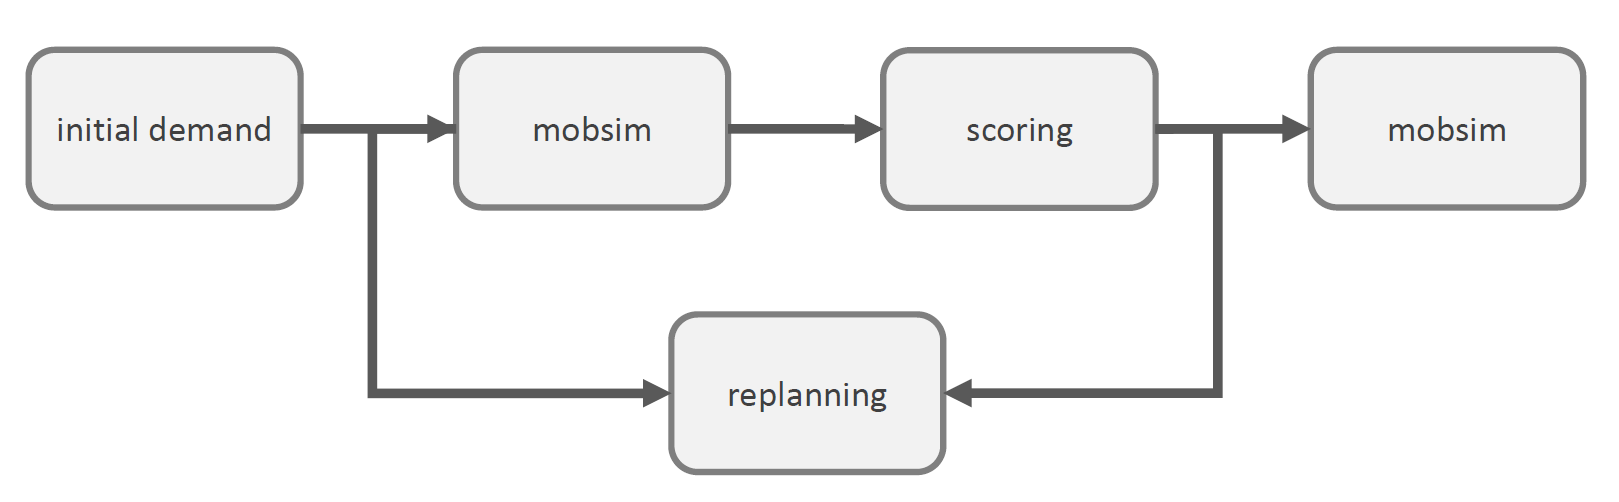
\includegraphics[width=0.95\textwidth]{images/matsim_loop.PNG}
    \caption{The MATSim cycle}
    \label{fig:matsim_loop}
\end{figure}


The \textit{initial demand} describes the full plan of activities, given as activity chains, for each of the agents. With each iteration, the individual agents try to optimise their initial demand. During the second building block, \textit{mobsim}, the individual agents execute their daily plans. Based on the performance of the selected plan, each agent scores the plan in the \textit{scoring} phase. The score is determined as a econometric utility function. This is followed by the \textit{replanning} building block. This phase allows agents to select a new plan. Each agent possesses a memory containing a configurable number of plans. The performance, or rather associated score, is also stored in the memory. Therefore, the agent selects a new plan based on the score previously allocated, during the \textit{mobsim} run, to the executed plan. Certain agents have the ability to modify the selected plan by cloning the plan and altering the certain dimensions of the plan. The most well known modifications available to the agent includes: adjusting the departure time, transport routes, selecting a different mode and changing the destinations.\par

The newly selected plan enters the second iteration of the \textit{matsim} loop and each agent executes the plan in the \textit{mobsim} run. If the number of plans stored in the memory should exceed the maximum allowable plans, the plan with the lowest score is removed from the agents memory. The \acrshort{matsim} cycle is repeated until the specified number of iterations is completed.  \par 

During the \textit{mobsim} run, the plan selected by each of the agents is executed on a road network that consists of different elements. The first is a link, which represents a segment of road. It is possible to set different parameters for each of the specified links such as the link capacity, the number of lanes, the maximum capacity, etc. The second element is a node. Nodes represent different locations in the network, given as a set of coordinates. Agents travel on different links to the node(s) set out in the selected plan. However, the agent is not the only agent travelling on the road network and has to compete with other agents. To accommodate for multiple agents travelling on a single link, \acrshort{matsim} has a built-in traffic flow model that adopts a queue-based approach to model vehicles entering and exiting certain segments of roads, in a certain road network.\par

\acrshort{matsim}'s plug-in architecture allows for various extensions to be contributed by other developers in the community. Since its development started in the 1990s by the Swiss Federal Institute of Technology, ETH Zurich \citep{horni2016multi}, the \acrshort{matsim} platform and the additional functionalities incorporated, has evolved to accommodate a large spectrum of problems and simulation scenarios. Such an extension includes the introduction of urban freight modelling in \acrshort{matsim}.\par

The inclusion of freight vehicles in \acrshort{matsim} has only recently been investigated. The first simulation of private and commercial vehicles on the smae road network, proposed by \citet{joubert2010large}, was achieved by using \acrfull{gps} data to construct activity chains for the freight vehicles. Similarly, the work done by \citet{joubert2011inferring} collected \acrshort{gps} data over a period of 6 months to construct the activity chains for commercial vehicle movement in South Africa. Further research in refining the activity chains used to simulate cmmercial vehicles in \acrshort{matsim} was conducted by \citet{van2014generating} and \citet{joubert2016freight}.\par

More recent developments include the introduction of the carrier and receiver agent into the \acrshort{matsim} framework \citep{schroeder2012towards, bean2020behavioural}. These extensions provide the capability to simulate logistic behaviour in \acrshort{matsim}. 

%--------------------------------------------------------------------------------------------------------------
\section{Modelling the carrier agent in MATSim}
\citet{schroeder2012towards} introduced a new software layer, the \textit{carrier} agent. This agent is responsible for the transportation of goods from a certain origin to a destination location. The carrier receives certain pick-up and delivery time windows during which he must complete his services at each of the receiver locations. Each carrier agent has a set of vehicles allocated to him. Each of these vehicles are tasked with a schedule that describes the list of receivers and the specified pick-up, delivery and arrival times, as planned by the carrier. The schedule also contains the planned route through the network.
Consider the extended \acrshort{matsim} cycle in figure \ref{fig:carrier_ext}. 

\begin{figure}[h]
    \centering
    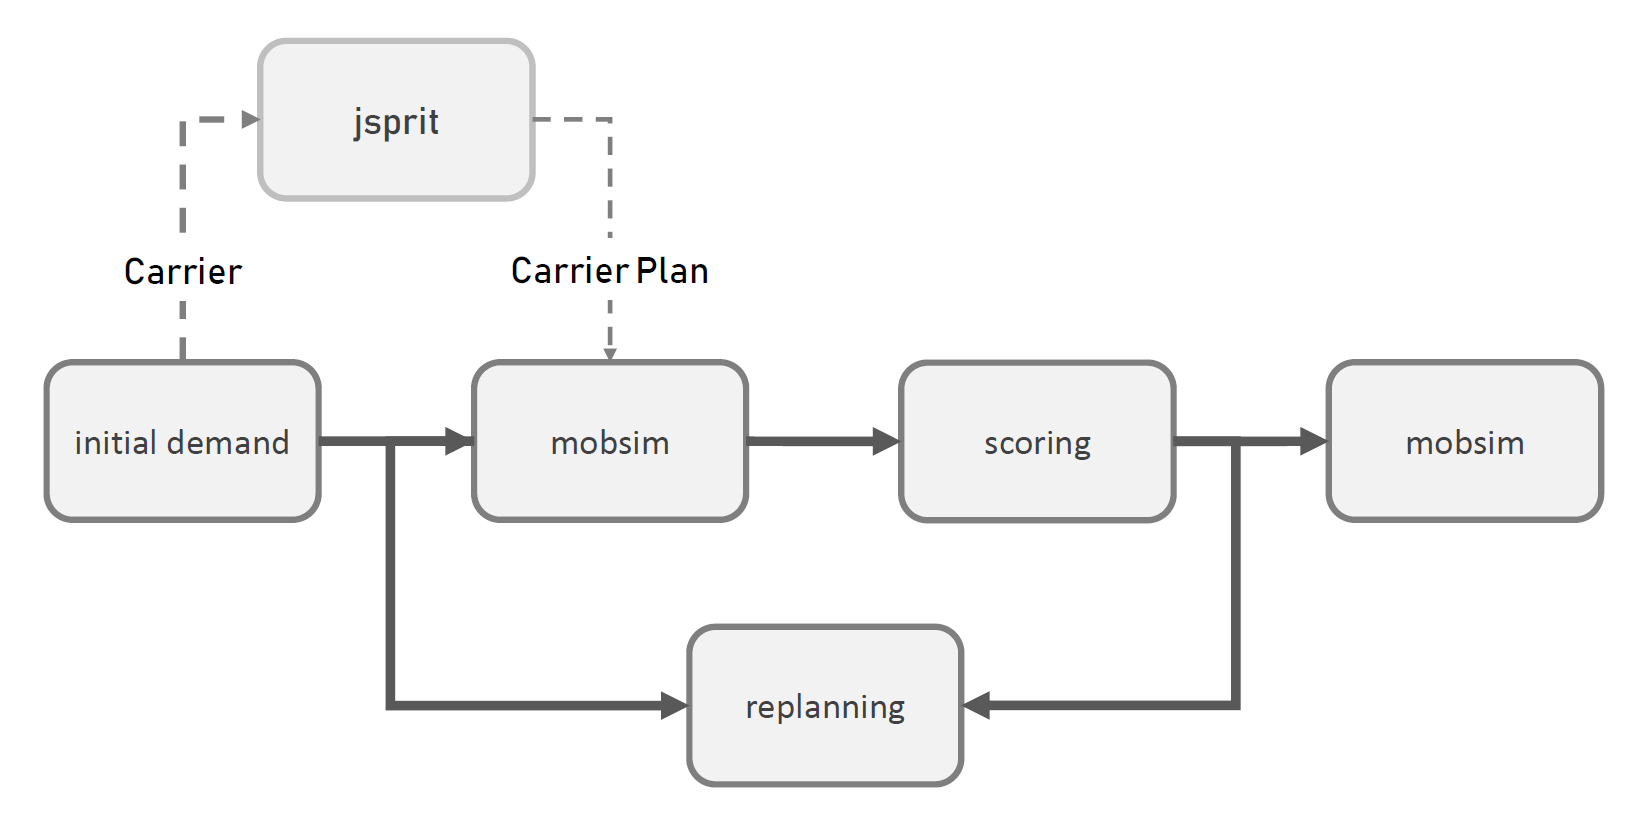
\includegraphics[width=0.95\textwidth]{images/carrier_extension.PNG}
    \caption{The MATSim cycle including the carrier extension }
    \label{fig:carrier_ext}
\end{figure}


To incorporate the carrier agent into this cycle, a toolkit called \texttt{jsprit} is used in conjunction with \acrshort{matsim}, as shown in figure XX. \texttt{jsprit} is an open source Java toolkit used to solve Vehicle Routing and Travelling Salesman problems \citep{jsprit}.  This figure was adapted from \citet{bean2020behavioural}. The \acrshort{matsim} and \texttt{jsprit} interface cycle also consists of five building blocks. Prior to executing the \textit{mobsim} stage, \texttt{jsprit} is called to construct the schedules for each carrier.  The carriers data container creates the interface with \acrshort{matsim} and \texttt{jsprit}. Figure \ref{fig:jsprit} provides a summary of the process steps and main process outputs obtained from the \texttt{jsprit} toolkit.\\

\begin{figure}[h]
    \centering
    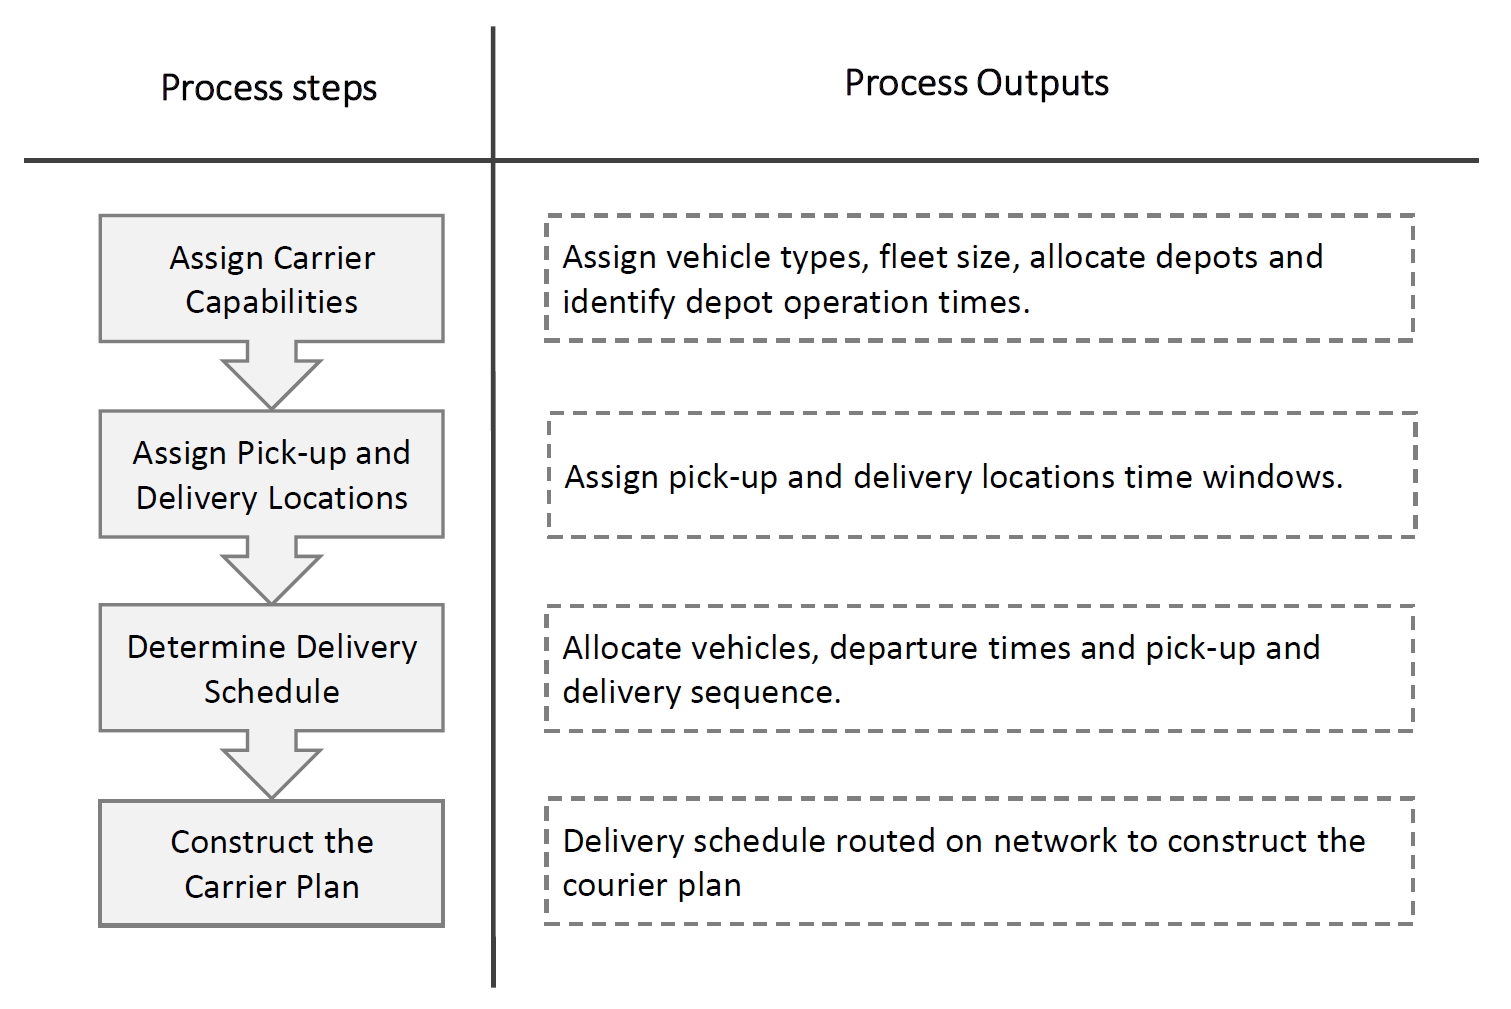
\includegraphics[width=0.95\textwidth]{images/jsprit_process.PNG}
    \caption{The \texttt{jsprit} process steps and outputs}
    \label{fig:jsprit}
\end{figure}


\paragraph{Assign carrier capabilities:} Each of these carriers are assigned certain capabilities when executing activities, including the different vehicle types and fleet size available to that carrier. 

\paragraph{Assign pick-up and delivery locations:} Each carrier operates from allocated depots, where each depot is assigned with a fleet size and vehicle type. This allocates certain vehicles to a certain depot location along with the specified depot operation times. Therefore, the carrier makes use of a variety of vehicles to perform pickup and delivery activities. If the carrier agent acts as both the carrier and the shipper, the depot location will act as the pickup location (shipper location). The carrier will only perform delivery activities in such an instance. All pickup and delivery activities are assigned a certain pickup and delivery time windows.

\paragraph{Determine delivery schedule:} Once the carrier capabilities and pickup and/or delivery time windows are assigned to each of the carriers, it is necessary to determine the delivery schedule, referred to as the tour schedule. The tour schedule contains the allocated vehicle, the planned departure times and the pickup and delivery sequence for each carrier. The carrier can combine different orders into a single vehicle, servicing all the relevant customers in a single delivery trip. However, a single order cannot be split into multiple freight vehicles. The pick-up and delivery sequence for multiple orders is determined by solving the Vehicle Routing and Travelling Salesman problem in \texttt{jsprit}. 

\paragraph{Construct carrier plan:} The resulting tour schedules are routed on the network to construct the routed tour schedules (referred to as the carrier plan) used by carrier agents to execute delivery activities in a single day. The completed carrier plan serves as the second interface between \texttt{jsprit} and \textit{matsim}. \\


The carrier plan is injected into the \textit{mobsim}, as indicated in figure \ref{fig:carrier_ext}. The agents travelling on the road network and executing assigned plans can be seen as individual drivers or rather a combination of a vehicle and a driver. One carrier agent can therefore have multiple vehicles travelling on the network.\par

Based on the carrier plan, each vehicle leaves its allocated depot at the planned time and travels on the network to the first customer stipulated on the list. The vehicle travels the shortest path on the network in order to save time and reduce the delivery cost. Each schedule contains the planned arrival time (delivery time) at the different receiver locations. The vehicle executes the deliveries at the different receiver locations, taking into consideration the allocated delivery time windows. Once all deliveries have been executed, the vehicle returns to the assigned depot location \par

After all plans have been executed by the different vehicles, the performance of the plans are evaluated and scored as an econometric utility function. After the \textit{scoring} stage has been completed, the carrier agent attempts to improve the performance of vehicles by altering the plans in the \textit{replanning} stage. The carrier will change the scheduling of the vehicles and switch the allocated deliveries between different vehicles in order to reduce the accumulated delivery cost. This process is repeated until the specified number of iterations is completed and the final stage, \textit{analyses} evaluates the performance of the different plans.

\section{Modelling the receiver agent in MATSim}
The receiver agent was implemented by following a similar framework to that presented by \citet{schroeder2012towards}. This agent is responsible for reordering goods and receiving deliveries from carriers. The receiver agent defines the order quantity (delivery size) and the delivery time window. For each of these parameters the receiver specifies certain criteria that have to be met by the carrier. These imposed requirements are referred to as the reordering requirements. The receiver behaviour was integrated into the existing framework of the carrier agents in \acrshort{matsim}. We refer once again to the \acrshort{matsim} cycle. Figure \ref{fig:receiver_ext} shows the updated \acrshort{matsim} cycle incorporating the carrier and receiver interaction. This figure was adapted from \citet{bean2020behavioural}.
\par

\begin{figure}[h!]
    \centering
    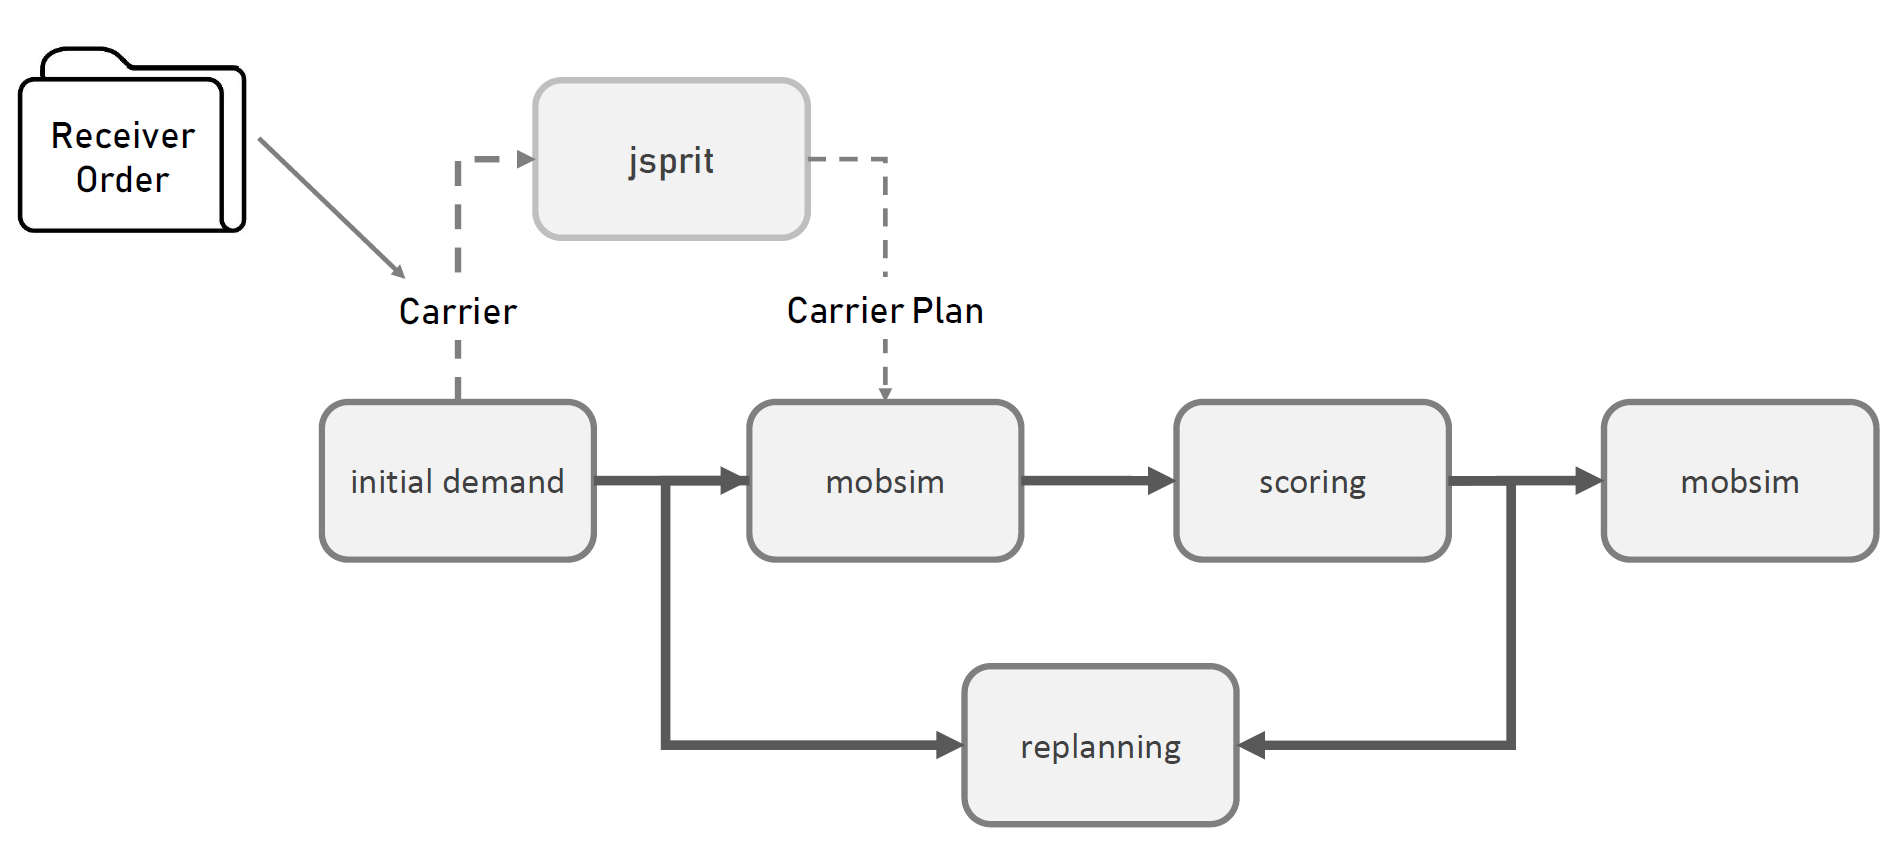
\includegraphics[width=0.95\textwidth]{images/receiver_extension.PNG}
    \caption{The MATSim cycle including receiver reordering behaviour }
    \label{fig:receiver_ext}
\end{figure}


\subsection{Initial demand}
During the \textit{initial demand} phase, a group of receiver agents are created. Each of these agents is assigned a facility location and added to the receiver data container. For each group of receivers, a list of product types are generated containing the product description and the capacity required to transport one unit of the product. The relevant product types are then allocated to the receivers. Each product type allocated to an individual receiver is also assigned an initial stock value. Based on these figures and the reordering policy, the daily reorder quantity is calculated and a new receiver order is generated. Each product type is replenished based on the assigned reordering policy.

\subsubsection{The reordering policy} 
The current policy in \acrshort{matsim} (implemented by \citet{bean2020behavioural}) is based on the \((s,S)\) reordering policy. The \((s,S)\) reordering policy determines the difference between the maximum inventory level, represented by \(S\), and the level of inventory currently available, below the minimum represented by \(s\). The output from the reordering policy, the weekly order quantity, is converted to a daily order quantity figure for the purpose of the single day simulation executed in \acrshort{matsim}. The proposed structure of the reordering policy allows for the incorporation of alternative reordering policies as it is extendable. Each order is assigned a unique order name, the required unloading time and the preferred number of weekly deliveries. The author does acknowledge the limitation of the single inventory policy. It is necessary to include other inventory policies into \acrshort{matsim}. The flexibility of the \acrshort{matsim} framework does allow for multiple policies to be incorporated. This is an important factor to consider as it does have an impact on the receiver reordering decisions and the resulting freight movement requirements. \par


\subsubsection{Adapting the single day simulation}
As \acrshort{matsim} simulates a single day, the number of weekly orders required will affect the volume to be delivered per day. A receiver requesting less than five deliveries a week, might not receive a delivery on the specific day simulated (if a five working day policy is assumed). To avoid the instance where a receiver receives zero cost allocation because of no delivery, the weekly delivery cost is estimated. The fixed costs, vehicle capacities, the carrier's cost of time and the number of weekly deliveries requested by the receiver is used to estimate the weekly delivery cost for each receiver.\par

\subsection{The \texttt{jsprit} interface}
Each generated order is then allocated to a specific carrier. A list of orders to satisfy is compiled for each carrier. The final initial plan allocated to each carrier agent is generated. In the instance where a single receiver requires deliveries from multiple carriers, it is included in this receiver plan. Each order is accompanied by the receiver specified delivery time windows. To integrate the generated receiver order into the existing carrier framework, the order is included as part of the carrier shipment list where the different vehicle types, pickup and delivery locations of the individual carriers are stored. As shown in figure XX, the receiver order is therefore added to the data injected into the \texttt{jsprit} toolkit prior to running the \textit{mobsim} stage. This list contains the unique order name, the receiver facility location, the preferred delivery time windows the size of the order (given in weight or volume) and the unloading duration. The receiver order (injected into the carrier shipment container) is rerouted and scheduled in \texttt{jsprit}.

\subsection{The mobsim}
From here, the carrier plan is generated for each of the carrier agents and set as the carriers' initial plan. These plans are then executed in the mobsim stage in the same manner as that discussed for the carrier agent in the previous section. \par

\subsection{Scoring}
Once the mobsim stage is completed, the process enters the next step in the \acrshort{matsim} cycle, the \textit{scoring} stage. Plans executed in the mobsim are scored using the econometric utility function. The calculated econometric function includes the delivery cost for each of the carriers. To translate these costs to the different receiver agents, the delivery costs are allocated proportionally to the different receivers served by the carrier. The proportional allocation of costs is the basic approached used, but the \acrshort{matsim} infrastructure can accommodate alternative methods. The allocation of costs are discussed in further detail in the following sections. The calculated cost allocated to each of the receivers from the carrier(s) can be seen as the score allocated to the specific plan executed by the different receivers and thus describes the performance of the plan. \par

\subsection{Replanning}
\label{replanning}
After the performance of the executed plan has been scored, the cycle enters the \textit{replanning} stage. After each iteration the carrier agent attempts to improve its own situation by altering its delivery plan to improve its performance. Similarly, each receiver agent will also attempt to improve its selected plan's score by reducing the total delivery cost allocated to him. The receiver replanning is done at the beginning of each iteration. This is done by introducing a replanning iteration variable into the framework. 

\subsubsection{The replanning iteration}
This variable is customisable by the modeller and describes after how many intervals the receiver agents are allowed to change their selected plans. If the simulation reaches the specified replanning iteration, the receiver agent has to decide whether its selected plan is sufficient or if any alterations are required. The receiver agent can change its specified plan by applying one of the different replanning strategies. This includes:
\begin{enumerate}
    \item Select the best plan from past plans based on the allocated score
    \item Adjust the delivery time window specified for the product type
    \item Adjust the delivery unloading time
    \item Adjust the delivery frequency 
\end{enumerate}

\subsection{The \texttt{jsprit} interface}
The new receiver order is injected into \texttt{jsprit} and a new carrier shipment is generated. The new carrier shipment includes the updated order quantity, delivery time windows and delivery unloading times. In \texttt{jsprit} updated plans are rerouted and a new schedule, the carrier plan, is injected into the mobsim stage. From here the cycle is completed and new scored are determined for these executed plans. The score allocated to the specific plan is stored in the agent's memory for future iterations.


%------------------------------------------------------------------------------------------------------------------------------------------------
\section{Modelling a receiver-driven collaboration}

The inclusion of the carrier and receiver software layers in \acrshort{matsim} enable the modelling of receiver-driven collaborations. \acrshort{matsim} accommodates the formulation of collaborations between the receiver and carrier agents. This extension was introduced by \citet{bean2020behavioural}. 

\subsection{Collaboration in urban freight transport}
Collaboration in the transportation sector can assist to reduce the environmental footprint, the number of trips required and increase the utilization and efficiency of delivery vehicles \citep{perez2015horizontal}. \citet{ballot2010reducing} focused on the complexity of the transport network between warehouses and distribution centres by pooling warehouses together. \citet{caputo1996internal} evaluated different policies between interacting agents such as standardizing pallets and documentation. Papers addressing the problem of fair cost allocation models were addressed by \citet{audy2012empirical}, \citet{houghtalen2007designing} and \citet{dai2012profit}. \citet{audy2012empirical} proposes using a network model to identify a stable collaboration group and makes use of Cooperative Game theory concepts to allocate costs. Similarly, \citet{houghtalen2007designing} addresses the fair allocation of benefits between carriers by implementing models based on Cooperative Game theory. Other articles explaining collaborative concepts in logistics and transportation environments and the resulting benefits from the collaboration include: \citet{janjevic2018investigating}, \citet{gonzalez2012defining}, \citet{lozano2013cooperative} and \citet{lindawati2014collaboration}. \citet{dai2012profit} made use of three Cooperative Game theory concepts based on the Shapley value, the proportional allocation concept and the contribution of each carrier. The paper studies the collaboration between carrier agents with pickup, delivery requests and time window constraints. The paper concludes by identifying future contributions as the development of practically implementing these solutions. \par

Including the behaviour of agents in a receiver-carrier collaboration can improve our understanding of designing and managing collaborations in industry.It can further assist in understanding the behaviour of individual agents when the collaboration costs are allocated among these agents. The available infrastructure in \acrshort{matsim} is investigated.

%Collaboration in urban freight transport is evident in literature, with a large body of literature focusing on the allocation of costs by incorporating concepts from cooperative game theory. Cooperative Game theory addresses not only the individual player but specifies the outcome of what a coalition could achieve when in agreement \citep{kuhn1997classics}.  Cooperative Game theory aids as a useful tool to evaluate scenarios where multiple players agree to form a collaboration with the condition that they obtain some form of benefit from collaborating \citep{ozener2008allocating}. This dissertation aims to support the inclusion of collaboration between urban freight vehicles by identifying the minimising the gap between the theoretical knowledge and the capability of the practitioners in the transport industry. \acrshort{matsim} facilitates the modelling of collaboration between the receiver and carrier agent as discussed in the next section. \par

\subsection{Urban freight collaboration infrastructure in MATSim}
\label{collaboration_infrastructure}
Following the inclusion of the carrier and receiver agent, \citet{bean2020behavioural} also implemented the required infrastructure to model carrier-receiver collaborations and cost allocations. The infrastructure embedded into \acrshort{matsim} are discussed below.

\paragraph{The coalition class:} An additional class was introduced into the \acrshort{matsim} framework. The \texttt{coalition} class describes the members that form part of a coalition instance. The members are shown as a collection of carrier and receiver agents. The different coalition instances include the grand coalition and other sub-coalitions. The latter describes coalitions that are not part of the grand coalition. To keep track of the collaboration status of the different receiver agents, alternative attributes are introduced.

\paragraph{The grandCoalitionMember attribute:} This attribute is set at the beginning of the simulation run and cannot be changed during the simulation. This attribute separates the receiver agents that are willing to form part of the grand coalition, from those that are not willing to form part of any coalition. The receiver agents that form part of the latter will be prohibited to form part of a coalition at any time in the simulation run.

\paragraph{The collaborationStatus attribute:} This attribute is also defined for each receiver agent and tracks whether the agent is collaborating at a specific time. The attribute is set as either \texttt{true} or \texttt{false}. This attribute is set to \texttt{true} if the receiver is part of the grand coalition. The attribute is set to \texttt{false} if the receiver is willing to collaborate (tracked by the grandCoalitionMember attribute) but not currently collaborating or if the receiver is not willing to collaborate under any circumstances and the receiver is not included in any form of coalition throughout the simulation.

\paragraph{A new replan startegy:} During the replanning stage, a replanning iteration is introduced that describes after how many intervals the receiver agents are allowed to modify their plans. The replanning iteration (discussed in section \ref{replanning}) allows certain receiver agents have the ability to change their selected plans. This replanning stage is, however, only available to the receiver agents that for part of grand coalition. Grand coalition members can make the individual decision to join or leave certain coalitions. 

\paragraph{The scoring phase:} The scoring phase scores the performance of the plan executed. The econometric function used to score the performance is different for collaborating and non-collaborating members. The receivers that do not form part of the grand coalition are charged a fixed cost. The fixed cost specified by \citet{bean2020behavioural} is given as a a rate per tonne, irrelevant of the distance travelled to serve the receiver. The receivers that form part of the sub-coalition are charged a variable cost.The allocation of this cost amongst the sub-coalition members depends on the cost allocation method used. The \acrshort{matsim} framework allows for multiple cost allocation methods to be included. In the contribution made by \citet{bean2020behavioural}, two cost allocation methods were embedded into the software. These include the proportional based on volume and the marginal cost allocation methods.

%Individual decisions are influenced by the consequences of these choices \citep{morrow1994game}. The social "structure" of an individual (referred to as a player) will influence what is perceived as the possible list of decisions, the impact of these decisions and how the player experiences or reacts to the outcome of a chosen decision. Game theory provides a framework to mathematically formalize these structures. The combination of the players' decisions lead to a certain outcome and these interrelated decisions are captured in Game theory \citep{morrow1994game}. Game theory regards these players as being "selfish" \citep{ozener2008allocating}. Each player will constantly adapt these decisions to improve their own situation \citep{wiese2010applied}.\par

\section{Cost allocation in urban freight collaborations}

In this section, the cost allocations available in literature are investigated. Before introducing the different cost allocation models, an introduction on cooperative Game theory concepts are provided. The section also delves into the literature on the models currently available in \acrshort{matsim}. The section concludes with a discussion on the applicability of the available models in practical scenarios.\par


Research shows that there is no single superior cost allocation method applicable to all collaborative scenarios. The selection of cost allocation methods is case-specific \citep{ouhader2017combining}. Literature does however indicate that the complexity of the cost allocation methods used does have an impact on the success rate of collaborative initiatives. Therefore, the resistance to collaborate lies not only on the uncertainty of the expected benefits and how these will be allocated but also on the complexity of the cost allocation models.\par

%--------------------------------------------------------------------

\subsection{Cooperative Game Theory Concepts}
According to \citet{branzei2008models}, a cooperative model between two or more players is presented by the pair (\textbf{N} , \textit{v}). \textbf{N} represents a finite set of potential players, where \textbf{N} = (1,...,\textit{n}). \textbf{N} also refers to the \textit{grand coalition}. The \textit{characteristic function} is given as \textit{v}(\textbf{S}). This represents the maximum worth, or in this case the maximum cot savings, of the coalition. The \textit{characteristics function} assigns the cost savings from coalition \textbf{S}, which is a sub-coalition of the grand coalition (\textbf{N}), to the cooperating players of this coalition. The subset \(\textbf{S}\subseteq \textbf{N}\) is in some instances referred to as a \textit{crisp coalition}. An empty coalition, where non of the players in set \textbf{N} make the decision to collaborate, is denoted by $\varnothing$. \par

To interpret these concepts, we refer to a simple example (example adapted from \citet{bean2019behavioural}). In this example, three players are identified. Player one receives a 2 tonne delivery on a Monday, whereas Player 2 receives his delivery on a Wednesday. Both players are situated in Boksburg, which falls under the Ekurhuleni District. Furthermore, both players are serviced by the same carrier, which is also Player 3 in this game, Carrier A. For each delivery made, Carrier A incurs a fixed and variable cost. Factors such as the cost of equipment, depreciation cost and insurance cost contribute to the fixed cost incurred. Variable costs include costs related to a specific delivery such as fuel and maintenance costs \citep{bean2019behavioural}.\par
Carrier A incurs the following variable costs for each player: Player A = R 800, Player B = R 500.

It is assumed that Carrier A owns a delivery vehicle with a capacity of 3 tonnes and incurs a fixed cost of R1500 with each delivery made. The original cost to service (prior to collaborating) is given as R800 + R500 + R1500 + R1500 = R4300. \par

If the players agree to receive the weekly delivery on the same day, Tuesday, Carrier A will only have to make use of one delivery trip to serve both players. This will require additional unloading time as Carrier A will have to unload at two facilities. It is assumed that the additional unloading time incurs a cost of R300 (cost of time). The outcome of the collaboration results in a reduction in the original delivery cost incurred, given as R800 + R500 + R1500 + R300 = R3100. For this example discussed, the characteristic function is shown in equation \ref{exNoCollab} and \ref{exAllCollab}.

Let \textbf{N} = (1,2,3) ; where n = 1 (Player 1); n = 2 (Player 2); n = 3 (Carrier A)
\begin{equation}
\label{exNoCollab}
    v\{\varnothing\} = V\{1\} = V\{2\} = V\{3\} = V\{1,2\} = V\{1,3\} = V\{2,3\}
\end{equation}

\begin{equation}
\label{exAllCollab}
    v\{1,2,3\} = 1200
\end{equation}

From this example, it is derived that the savings (also referred to as gain) are only realised if all players in coalition \textbf{S} form part of the collaboration. Therefore, the players cannot save on the delivery cost incurred if any sub-coalition is formed. \citet{branzei2008models} explains a similar phenomena in an example referred to as the \textit{Glove Game}.\par

Cooperative Game theory allocates the savings by firstly identifying the characteristic function, as described above. This is followed by coalition function that determines the payoff to each player in the coalition. To ensure the fairness of this allocation, it is governed by certain properties referred to as axioms \citep{hadzic2013cooperative}. \citet{defryn2013gain} summarizes the most valuable axioms as follows:

\paragraph{Efficiency}: This condition ensures the cost allocation methods distributes the entire cost amongst players. Let \(\emph{x} = (x_1, x_2, ..., x_n)\) be the vector that allocates a cost of \(x_i\) to player \textit{i} in the coalition \emph{N}. The \textit{efficiency} condition is expressed in formula \ref{efficiency}.
\begin{equation}
\label{efficiency}
\sum_{\substack{i\in N}} x_\textit{i} = \textit{v} (\textbf{N})
\end{equation}

\paragraph{Individual rationality}: The cost allocated to a collaborator cannot be less beneficial by joining the coalition, than the cost of acting alone. This property ensures that a player joining a coalition is not worse off than before joining. If this property is adhered to, each player is assigned a positive profit. Where \( c({i})\) represents the cost allocated to player \textit{i} if he decides not to collaborate, but rather act alone. This equation is given in equation \ref{individualrationality}.
\begin{equation}
\label{individualrationality}
x_i \geq \textit{v}(i) \quad \forall \quad i \in \textbf{N}
\end{equation}

\paragraph{Stability}: Partners cannot improve their current situation by forming a sub-coalition. This means that the cost allocation method ensures individual rationality for every possible sub-coalition and each player is assigned a positive profit. The stable cost allocations are referred to as being in the \textit{core}. This allocation provides stability as no player could increase their gain by deviating from the \textit{grand coalition}. If the cost allocations are not in the \textit{core}, it is defined as being unstable. Players might choose to form part of a sub-coalition instead of the grand coalition if they could achieve greater benefits, and the coalition might dissolve. The stability axiom is given in equation \ref{stability}.
\begin{equation}
\label{stability}
\sum_{\substack{i\in S}} x_\textit{i} \geq v (\textbf{S}) \quad \forall \quad S \subseteq \textbf{N}
\end{equation}

\paragraph{Additivity}: The allocation of costs is not affected by partners forming larger coalitions. The cost allocated to two individual players is the same as that allocated to the sum of the two players. If a game is separated into two parts and for any two values allocated (\(v_1\quad and \quad v_2\)) the game for every coalition S is defined by equation \ref{additivity}.

\begin{equation}
\label{additivity}
    ( v_1 + v_2 )(\textbf{S}) = v_1(\textbf{S}) + v_2(\textbf{S}) 
\end{equation}

\paragraph{Dummy player}: A player that does not contribute but does not negatively impact the coalition, receives an allocation of zero. Therefore, if \textit{i} represents a \textit{dummy player}, the contribution made by \textit{i} is 0 for all subsets. This means the value of a coalition with player \textit{i} is the same as the value resulting from the coalition without \textit{i} and the condition is mathematically written as shown in equation \ref{dummyplayer}.

\begin{equation}
\label{dummyplayer}
    v(\textbf{S} \in {i}) = v(\textbf{S}) \quad \forall \textbf{S}\
\end{equation}


Research identifies multiple cost allocation methods. No single method possesses all the properties \citep{defryn2013gain}.  In the next section, various of the existing most allocation methods will be discussed. Table XX summaries the properties possessed by each of these methods. 
%----------------------------------------------------------------------

\subsection{Cost Allocation Methods}
To ensure the stability of a collaboration it is critical to understand the \textit{pain and gain sharing} within the transportation scenario  \citep{savelsbergh201650th}. The importance of understanding these cost allocation models have been discussed by various other papers in the last decade \citep{gonzalez2012defining,guajardo2016review,janjevic2018investigating,lozano2013cooperative}. \citet{janjevic2018investigating} describes the term "gain" as being the reduction in cost resulting from a certain cooperative model. Therefore in a cost allocation model, the gain is seen as the reduction in the cost of collaborating compared to the cost of acting alone. The literature study on cost allocation methods identifies the frequently used methods, applications thereof and the benefits and limitations of applying each.

\subsubsection{Proportional Method}
As the name entails, the proportional method links the gains, generated from a coalition, proportionally to the relevant contributor \citep{janjevic2018investigating}.  
In the proportional method, each player is assigned a specific share of the total cost \citep{ouhader2017combining}. These shared values are assigned to the players based on a certain set of criteria \citep{ouhader2017combining} and the chosen criteria link the gains to a single indicator \citep{janjevic2018investigating}. The simplest form of the proportional method is known as the \textit{Egalitarian  method} where shares are allocated equally amongst the players. Other known criteria include the demand quantities and also stand-alone costs \citep{guajardo2016review}.\par

 The proportional method based on stand alone costs is given in equation \ref{proportionalA} and \ref{proportionalB}
 \begin{equation}
 \label{proportionalA}
 x_j = w_j c(\textbf{N})
 \end{equation}
 
 \begin{equation}
 \label{proportionalB}
  where \quad w_j = c({j}) \setminus \sum_{\substack{i\in n}} c({i})
 \end{equation}

The cost allocation to player \textit{j} is determined by a certain weight \( w_j\). This weight is calculated as the portion of stand-alone costs contributed by player \textit{j} compared to the sum of the cost contributed by each player in the grand coalition.

This method is one of the preferred methods in practice as it is easy to communicate with practitioners \citep{guajardo2016review}.
There is however evidence in the literature of its limitations. \citep{guajardo2016review} describes this method as showing signs of weakness. Applying the proportional rules in cost allocation methods does not guarantee a cost allocation that allocates the benefits in an equal and fair manner \citep{lozano2013cooperative}. Due to its ease of implementation, it is still considered as an option for allocating costs.   

\subsubsection{Separable and non-separable costs}
This method divides the cost to be distributed amongst the players, into two parts: the separable cost and the non-separable cost. This method allocates cost by first distributing the separable cost to each participant. Once this is done, the non-separable cost is then allocated to the players, according to a certain weight assigned to each player \citep{frisk2010cost}.  The separable cost is referred to as the marginal cost of player \textit{j} and is given as:
\begin{equation}
m_j = c(\textbf{N}) - c(\textbf{N} - (j))
\end{equation}
 The non-separable costs are distributed according the the weights chosen. The equation for determining the non-separable costs is given as:
 \begin{equation}
 g(\textbf{N}) = c(\textbf{N}) - \sum m_j.
 \end{equation}

The literature identifies various methods to assign weights to the distribution of non-separable costs, this paper will discuss two of the methods. The first is by simply allocating the cost evenly amongst players. This method is called the \textit{Equal Charge Method}. The second method is the \textit{Alternative Cost Avoided Method} where weights are assigned based on the savings made by player \textit{j} when joining the coalition. The weights are given as: \( w_j = c(j) - m_j\)

\subsubsection{Shapley Value}
Before allocating the costs it is necessary to clarify what is described as being "fair". In an attempt to describe "fairness", literature has identified four axioms (similar to the game theory properties listed by \citep{ozener2008allocating}). The Shapley Value Method satisfies these four axioms namely efficiency, symmetry, dummy property and additivity that results in a unique solution \citep{guajardo2016review}.\par

The Shapley Value was developed in 1953 by Shapley \citep{ouhader2017combining}. It is known as one of the most used concepts in cooperative game theory \citep{ouhader2017combining}.
The Shapley Value Method considers the participants', also referred to as the players', contribution to the main coalition as well as all the possible sub-coalitions in the game \citep{ouhader2017combining}. The coalition formation is done sequentially. The additional costs contributed by each joining partner is considered in all possible permutations and shared in a 'fair' manner \citep{defryn2013gain}. 

The contribution made by each player is defined as the weighted average of the marginal contribution. This includes all the different coalitions the player could participate in the game \citep{ouhader2017combining}. The average marginal value is described as the value each member would bring to the coalition if they were to enter it \citep{ozener2008allocating}. This method ensures gains are allocated in a fair manner \citep{janjevic2018investigating}.


An advantage of this method is that the result is unique. A disadvantage is that it does not belong to the core \citep{guajardo2016review}. Even if the core is found to be non-empty, the Shapley may not be included \citep{ozener2008allocating}.

Literature validates the use of the Shapley Value as a successful cost allocation method. The method has been used by the \(CO^3\) project in Europe \citep{defryn2013gain}. \citet{ozener2008allocating} conducted a study on the benefits of merging transportation activities of different companies to analyze the behaviour of different cost allocation methods. Another study by \citet{janjevic2018investigating} investigated characteristics shown by different gain sharing methods by applying it to a specific scenario in the Brussel Capital Region. It was concluded that the Shapley value offers the best compromise between the two characteristics investigated, namely rationality and stability requirements.
\citep{guajardo2016review} describes the Shapley Value method as one of the most frequently applied methods in cost allocation in cooperative game theory, especially in the field of collaborative transportation problems.\par

The cost allocation to each partner \textit{i} in the coalition is calculated with the equation \ref{shapley}.
 
\begin{equation}
\label{shapley}
\begin{split}
x_i= \sum_{\substack{\textbf{S}\subseteq \textbf{N}\\i}} \frac{|\textbf{S}|!(|\textbf{N}| - |\textbf{S}| - 1)!}{|\textbf{N}|!}(c(\textbf{S}\cup i) - c(\textbf{S}))
\end{split}
\end{equation}

\textbf{N} represents the number of players and \(c(\textbf{S} \in i)\) represents the cost with player \textit{i} included and \( c(\textbf{S})\) is the cost of the coalition \textbf{S} without player \textit{j} included. \((|\textbf{N}| - |\textbf{S}| - 1)!\) represents the number of ways the different players could have been added. \(|\textbf{S}|!\) is the number of ways set \textbf{S} could have been formed before player \textit{i} is added.


\subsubsection{Nucleolus}
In some scenario's there exists more than one cost allocation in the core. Some of the allocations present might be more preferable than others. The nucleolus is such a cost allocation that is well studied in literature \citep{ozener2008allocating}.
The Nucleolus method was introduced by Schmeidler in 1969 \citep{ozener2008allocating}. This method was originally defined as a profit game but was adapted to satisfy the requirements of a cost-sharing game  \citep{guajardo2016review}.
This method determines the optimal allocation of cost by lexicographically maximizing the minimal gain \citep{ozener2008allocating}. \citet{guajardo2016review} describes the minimal gain as the excess vector, where the excess in a game is a measurement by the satisfaction of such a certain coalition. The excess vector given by the equation \ref{nucleolus} measures the "happiness degree" of the coalitions \citep{lemaire1984application}.
\begin{equation}
\label{nucleolus}
e(x,\textbf{S}) = c(\textbf{S}) - \sum_{\substack{i\in \textbf{S}}} X_i
\end{equation}

A negative excess vector describes an allocation that does not belong to the core. A positive value assumes the core exists \citep{tanczos2005analysis}. This method maximizes the savings of the game (or the excess vector) to minimize the worst equity, rather than finding the fairest allocation \citep{janjevic2018investigating}.

Benefits of the nucleolus, that make its application as the chosen cost allocation method appealing, is its uniqueness \citep{guajardo2016review} and its inclusion in the core, even if the core is non-empty \citep{ozener2008allocating}. The computations of applying the nucleolus are more complex than methods that are based on formulas \citep{guajardo2016review} as several linear programs are computed and solved \citep{defryn2013gain}.
In an attempt to find the nucleolus and simplifying this process, many algorithms have been developed. Behiringer introduced a concept to solve the nucleolus in a cooperative game. Based on this Sankaran developed a way of solving the nucleolus for an n-person-game in his master's thesis. Both algorithms reduce the nucleolus complexity by solving a sequence of linear programs. An analysis of over games confirmed Behiringer's algorithm as being the superior solution of the pair \citep{fromen1997reducing}.\par

Although the results obtained from this method is favourable, the implementation thereof is difficult in real life scenario's as it is computations are difficult and requires the help of algorithms to solve.

\subsubsection{Equal Profit Method}
The Equal Profit Method, proposed by \citet{frisk2010cost}, allocates the relative savings in an equal manner. The method aims to minimize the greatest difference obtained by partners. The savings are allocated relative to the importance of the partner. The partners' stand-alone cost is used to define this importance \citep{defryn2013gain}. Limitations of this method are that it is only defined for a non-empty core. The uniqueness of a solution is not guaranteed \citep{wiese2010applied}. However, \citet{frisk2010cost} proposed this method as it provides a solution that minimizes the difference between the relative savings and serves as a good model to use in negotiations as it provides a stable solution. The following computations were also adapted from \citet{wiese2010applied}.
For player \textit{i}, the relative saving is expressed as shown in equation \ref{relativesaving}. The difference in relative savings between two players, \textit{i} and \textit{j} are given by equation \ref{equalprofitmethod}. The allocation according to the \textit{Equal Profit Method} is given in equation \ref{epmA}, \ref{epmB} and \ref{epmC}.
\begin{equation}
\label{relativesaving}
\frac{c({i}) - y_i}{c({i})} = 1 - \frac{y_i}{c({i})}
\end{equation}

\begin{equation}
\label{equalprofitmethod}
\frac{y({i})}{c({i})} = \frac{y_j}{c({j})} \quad \forall \quad  (i,j),
\end{equation}

\begin{equation}
\label{epmA}
\textit{f} \geq \frac{y_i}{c({i})} - \frac{y_j}{c({j})} \quad  \textbf{S} \subset \textbf{N}, 
\end{equation}

\begin{equation}
\label{epmB}
\sum y_i \leq c(\textbf{S}) \quad textbf{S}  \subset \textbf{N},
\end{equation}

\begin{equation}
\label{epmC}
\sum y_i \leq c(\textbf{N})
\end{equation}

\subsection{Cost allocation methods available in \acrshort{matsim}}
The scoring function in \acrshort{matsim} is modified to incorporate the allocation of cost. The following framework was introduced by \citet{bean2020behavioural}. During every iteration, the costs are allocated to the members that form part of the coalition (refer to section \ref{collaboration_infrastructure} for the coalition class and attributes that track the collaboration status of each receiver). The coalition cost, given as \(C(S)\), is determined as a function of the non-collaborating members and the total delivery cost incurred by the carrier. The calculation for the coalition cost is given in equation \ref{eq:coalition_cost}. Set \(C\) represents the carriers and \(N\) represents the non-collaborating receivers. 

\begin{equation}
\label{eq:coalition_cost}
    C(S) = \sum_{\substack{c\in C}} C_c^T - \sum_{\substack{c\in C}} F_c ( \sum_{\substack{n\in N}} V_{r_c} ^N)
\end{equation}

The second part of equation \ref{eq:coalition_cost} calculates the total amount paid to non-collaborating members. This is given as the volume of non-collaborating receiver, \(r\), transported by carrier, \(c\), multiplied by the fixed fee allocated per volume unit transported. The coalition cost, \(C(S)\), is allocated to the coalition members based on a specific cost allocation method. \acrshort{matsim} provides two cost allocation methods to allocate the costs calculated by equation \ref{eq:coalition_cost}. Each of these methods are discussed below.

%-----------------------------------------------------------------------------------
\subsubsection{The proportional method}
The Proportional method allocates the coalition cost based on the volume delivered to the receiver. The proportional cost allocated to each receiver, \(r\), by carrier, \(c\), is determined by equation \ref{eq:prop_cost}. The proportion of volume delivered to receiver, \(r\), by carrier, \(c\), of the total volume delivered by carrier, \(c\), is multiplied by the total delivery cost incurred by the carrier, \(c\). The total volume delivered by carrier, \(c\), is calculated by summing the individual deliveries ade to the set of receivers, \(r\), by the carrier as shown in equation \ref{eq:prop_volume}. Finally, the delivery cost allocated to each receiver, \(r\) is given as the summation of the delivery costs charged by all carriers, \(c\), serving the specific receiver. 

\begin{equation}
\label{eq:prop_cost}
    C_{r_c} = C_c ^T ( \frac{V_{r_c}{V_c^T})
}{V_c^T})
\end{equation}

\begin{equation}
\label{eq:prop_volume}
    V_c^T = \sum_{\substack{r \in R}} V_{r_c}
\end{equation}

\begin{equation}
\label{eq:prop_cost_receiver}
    C_r = \sum_{\substack{ c \in C}} C_{r_c}
\end{equation}

%-----------------------------------------------------------------------------------
\subsubsection{The marginal method}
The marginal cost allocation method calculates the coalition cost allocated to each member as a function of the grand coalition delivery cost and the delivery cost incurred by a sub-coalition containing all the grand coalition listed members except the specific member. The inclusion of this method into the \acrshort{matsim} framework deems more difficult than that of the Proportional method. This is due to the various instances that need to be executed in parallel to determine the costs incurred for each of the possible sub-coalitions. \citet{bean2020behavioural} includes this logic by duplicating the specific simulation instance into various branches, each branch representing the different sub-coalition. We refer to our example. Ruben and Thomas are the two receivers being serviced by the carrier, The Courier Guy. For a specific simulation instance, \(t\), the marginal method duplicates the instance and separates it into four different branches as shown in figure \ref{fig:marginal_example}. 


\begin{figure}[h]
    \centering
    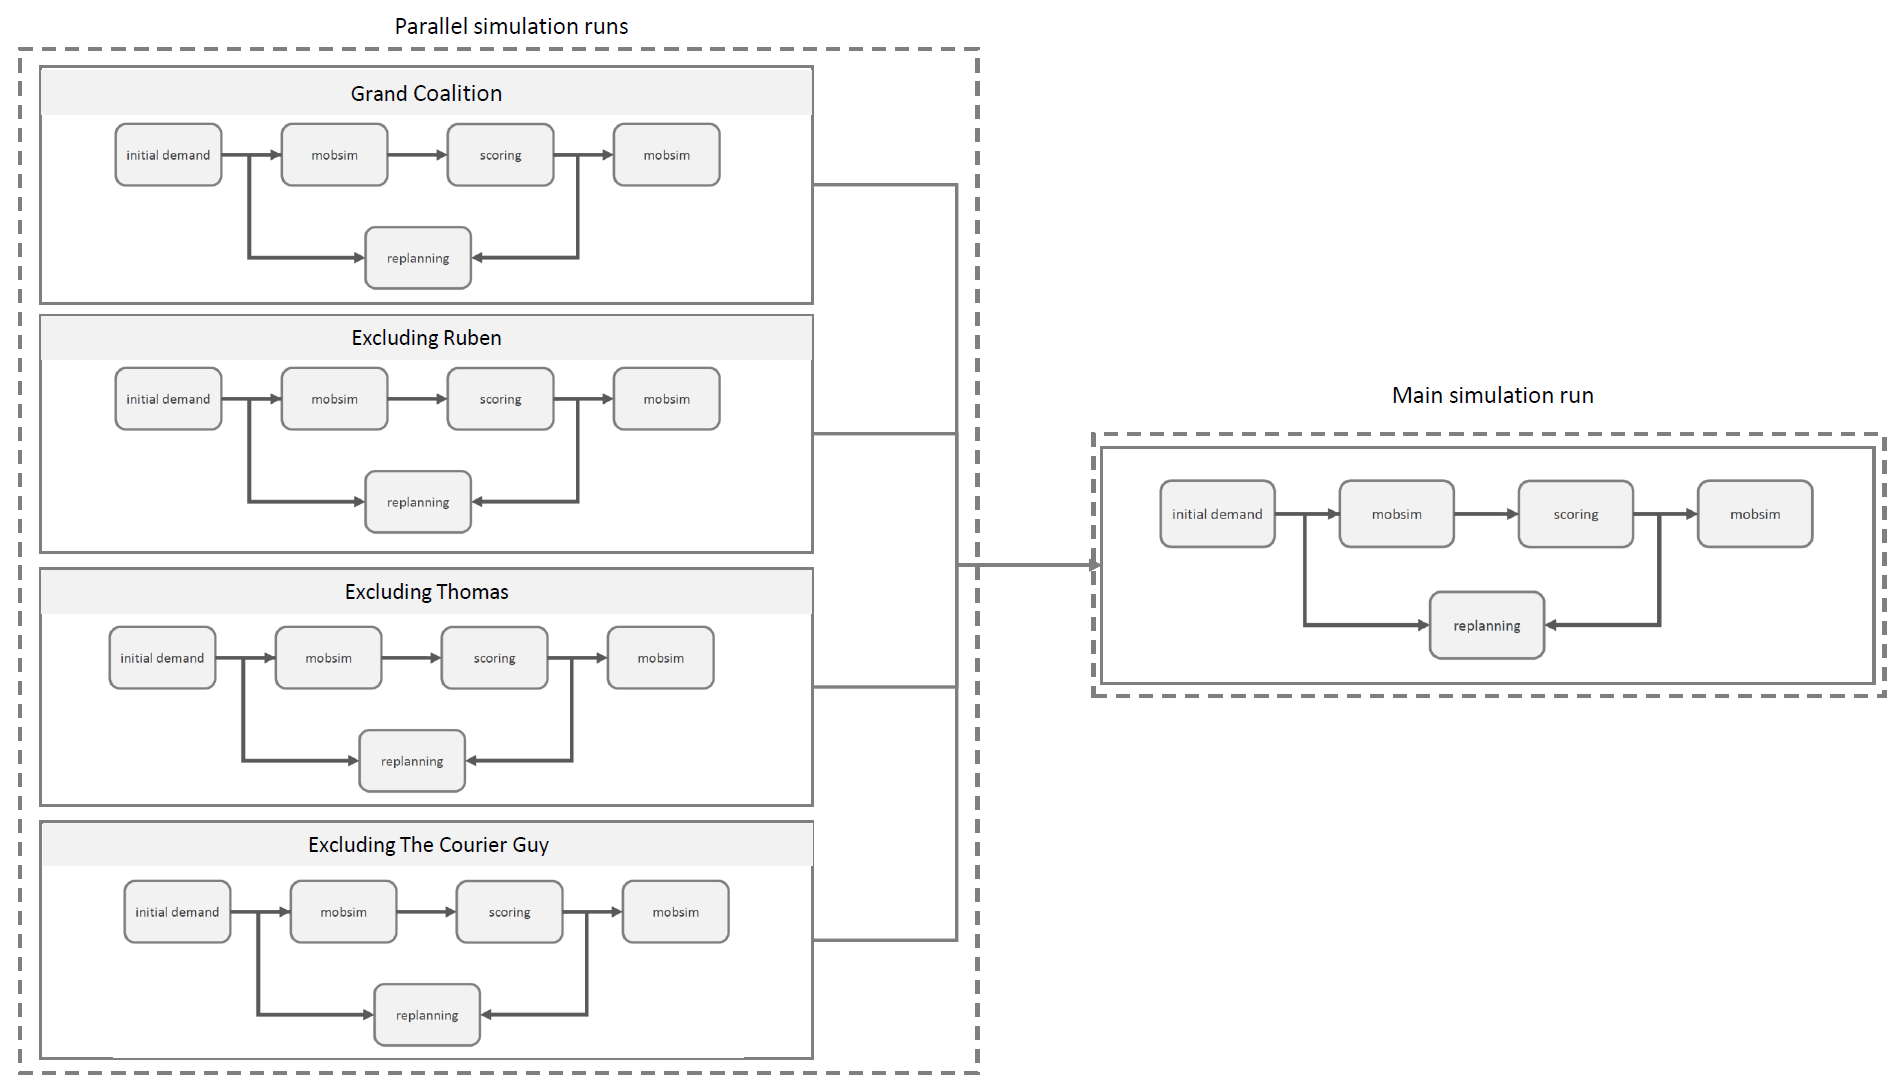
\includegraphics[width=1\textwidth]{images/marginal_example.PNG}
    \caption{An example of the marginal methods' parallel simulation}
    \label{fig:marginal_example}
\end{figure}

The first branch describes the grand coalition, where all the members form part of the coalition. In the second branch, Ruben is excluded form the sub-coalition. The third branch excludes the second receiver, Thomas, whereas the last branch excludes The Courier Guy. Each of the parallel streams executes a simulation run, as shown by the \acrshort{matsim} loops included in figure \ref{fig:marginal_example}. This is executed in an independent Java virtual machine. For each of the parallel branches, the coalition cost is determined by equation \ref{eq:coalition_cost}. The calculated coalition costs are then included in the main simulation run, as shown in figure \ref{fig:marginal_example}. The calculated coalition costs for the different parallel branches are stored as an attribute. These attributes are updated, at the end of each iteration, with the newly calculated delivery cost values.
The parallel simulation run is executed for every receiver replanning iteration during the simulation. The marginal cost, given as \(C_i^m\), allocated to each of the coalition members, \(i\), is calculated by equation \ref{eq:marginal_cost}. 

\begin{equation}
\label{eq:marginal_cost}
    C_i^ m = C(N) - C( N\{i\}) \quad \forall i \in \{1,...,N\}
\end{equation}

%--------------------------------------------------------------------------------------
\section{Areas for improvement}

The performance of the proportional- and marginal cost allocation methods are investigated by running a small scenario. The scenario included one carrier servicing six receiver agents on a small network. The simulation included 200 iterations to accommodate for variability. The case study evaluated the impact of the proportional based on volume cost sharing methods on the resulting reordering decisions made by the receiver. The three receiver dimensions, delivery time window, delivery unloading time and delivery frequency were altered and the results evaluated. The results indicated that receivers were more willing to form part of the coalition if the coalition cost was lower than the fixed fee. This is understandable as the autonomous behaviour of the agents will attempt to minimise the delivery cost incurred. \par

The results exhibit the change in receiver reordering behaviour when alternative cost allocation methods are applied. This emphasizes the importance of including a cost allocation method that allocated the cost in a fair manner that would increase the attractiveness of forming part of the coalition. The proportional method based on volume is known for its simplicity and is therefore a well known method as it is easy to implement. The results from the method are however limiting as some coalition members benefit more from the collaboration than others. This method favours members that require higher volumes than the receivers with small delivery quantities. This could result in potential members rejecting the idea of collaborating as it is perceived as being unfair.\par

The second cost allocation model, the marginal method, provides a more mathematical means of calculating the coalition costs allocated to the different receivers. The complexity of the model does, however, present limitations when implemented in \acrshort{matsim}. The parallel simulation runs require more dynamic computations to capture the receiver reordering behaviour without exponentially increasing the computational complexity of the model. \par

The cost allocation models in \acrshort{matsim} to model the collaboration between urban freight vehicles pose limitations. Although these models serve as an excellent starting point in modelling realistic collaborations, further research is required to refine these cost allocation models. The attractiveness of entering a coalition lies heavily on the performance of the cost allocation model. It is therefore imperative that the \acrshort{matsim} framework present models that are fair, validated and applicable to practical scenarios in industry.\par 

Furthermore, the results described by \citet{bean2020behavioural} indicate that the members were less willing to collaborate if marginal cost allocation method was used as the coalition cost often resulted in higher delivery cost than that of the fixed fee allocated to the non-collaborating members.
%---------------------------------------------------------------------------------------------------------------------------------------------------------------------------------------------------------------------------------------------------------------------------
%\section{Areas for improvement}
%The \acrshort{matsim} framework does allow the modelling of receiver-carrier collaborations. The contributions made by \citet{bean2020behavioural} provides the necessary tools to model a collaboration as well as allocate the resulting costs among the collaborating partners. Although \acrshort{matsim} has the capability of simulating realistic collaboration scenarios, there are, however, limiting factors included in the model. The first lies within the replanning iteration of the model. As noted by the author, the reordering inventory policy cannot capture the reordering behaviour of different receivers in industry. Bean suggests future research should expand this area of research by incorporating additional models such as the \acrfull{eoq}.\par

%A second limitation of the available model 


%\subsection{Investigation of available cost allocation methods}



%\subsection{Allocation of fixed fees}

















%\section{Conclusion}
